\documentclass[11pt]{article}
\usepackage{epsfig}
\usepackage{float}
\usepackage{longtable}
\restylefloat{figure}
\restylefloat{table}
\usepackage[margin=0.75in]{geometry}
\usepackage{hyperref}
\usepackage{fancyhdr}
\pagestyle{fancy}
\lhead{ARM RCE Generation 3 Core Module}
\rhead{Design Document}
\lfoot{Version 1.2}
\rfoot{\thepage}
\cfoot{}

\begin{document}
\thispagestyle{empty}

\title{ARM RCE Generation 3 Core Module \\ Design Document}
\author{Ryan Herbst}
\date{\today}

\maketitle
\begin{table}[H]
\centering
   \begin{tabular}{| l | l | l | l | } 
      \hline \textbf{Revision} & \textbf{Effective Date} & \textbf{Description Of Changes} \\
      \hline 1.2               & April 2, 2014       & Updates for local bus to AXI-Lite conversion.  \\
                               &                     & PPI interface changes.  \\
                               &                     & Some document sections removed. \\
      \hline 1.1               & November 14, 2013       & Added clock select registers.  \\
      \hline 1.0               & November 8, 2013        & Cleanup.  \\
      \hline 0.3               & November 5, 2013        & Changed location of outbound free list FIFOs.  \\
      \hline 0.2               & October 24, 2013        & Cleaup, additional functional descriptions. IB/OB descriptor updates. \\
      \hline 0.1               & October 22, 2013        & Initial revision                \\
      \hline
   \end{tabular}
\end{table}

\vfill
\begin{center}
SLAC National Accelerator Center
Research Engineering Division, Electronics
\end{center}
\newpage
\tableofcontents

\newpage
\listoftables

\newpage
\listoffigures

\newpage
\section{External Interfaces}
\label{sec:external_interfaces}

This section of the document describes the external interfaces of the ARM RCE generation 3 core module. See
table \ref{tab:top_signals} in section \ref{subsec:ArmRceG3Top} for a detailed list of the top level interface signals.

\subsection{External Clock \& Reset}
\label{subsec:external_clock_reset}

The following table defines the clock and reset signals output from the ARM RCE generation 3 core module.

\begin{table}[H]
\small
\centering
   \begin{tabular}{| l | l | l | }
      \hline \textbf{Signal} & \textbf{Description} \\
      \hline axiClk          & AXI Bus clock. Nominal 125Mhz. Used to clock AXI-Lite bus signals.      \\
      \hline axiClkRst       & Reset strobe synchronous to axiClk.                                  \\
      \hline sysClk125       & 125Mhz system clock.  \\
      \hline sysClk125Rst    & Reset strobe synchronous to sysClk125.                               \\
      \hline sysClk200       & 200Mhz system clock.  \\
      \hline sysClk200Rst    & Reset strobe synchronous to sysClk200.                               \\
      \hline
   \end{tabular}
   \caption{External Clock \& Reset Signals}
\end{table}

\subsection{External AXI-Lite Bus}
\label{subsec:external_axi_bus}

Contained within the RCE core module is a AXI to to AXI-Lite bridge that facilitates register read and write access within the core. 
This controller described in section \ref{subsec:ArmRceG3LocalAxi} of this document allocates a portion (0xA0000000 - 0xBFFFFFFF) of the AXI-Lite address space to an external AXI-Lite bus. The read and write portions of this bus operate independently, allowing simultaneous read and write access. Support logic for interfacing to this bus can be found in the axi sub-section of the SLAC RED Electronics standard VHDL library. Four record types, 2 for write and 2 for read, make up the AXI-Lite bus. For more information about Axi-Lite bus transactions, please see AMBA AXI Protocol Specification.

The first record type, AxiLiteReadMaster is an output containing the following signals:

\begin{table}[H]
\small
\centering
   \begin{tabular}{| l | l | l | }
      \hline \textbf{Signal} & \textbf{Width}  & \textbf{Description} \\
      \hline araddr          & 32              & Read address vector.                         \\
      \hline arprot          & 2               & Read protection value. (usually not used).    \\
      \hline arvalid         & 1               & Asserted when araddr and arprot are valid.   \\
      \hline rready          & 1               & Asserted when master is ready to accept read data. \\
      \hline
   \end{tabular}
   \caption{AXI Lite Read Master Record}
\end{table}

The second record type, AxiLiteReadSlave is an input containing the following signals:

\begin{table}[H]
\small
\centering
   \begin{tabular}{| l | l | l | }
      \hline \textbf{Signal} & \textbf{Width}  & \textbf{Description} \\
      \hline arready         & 1               & Asserted when slave is ready to accept a read transaction. \\
      \hline rdata           & 32              & Read data vector.                         \\
      \hline rresp           & 2               & Read response vector. Indicates status of read transaction. \\
      \hline rvalid          & 1               & Asserted when read data and response are valid. \\
      \hline
   \end{tabular}
   \caption{AXI Lite Read Master Record}
\end{table}

The third record type, AxiLiteWriteMaster is an output containing the following signals:

\begin{table}[H]
\small
\centering
   \begin{tabular}{| l | l | l | }
      \hline \textbf{Signal} & \textbf{Width}  & \textbf{Description} \\
      \hline awaddr          & 32              & Write address vector.                         \\
      \hline awprot          & 2               & Write protection value. (usually not used).    \\
      \hline awvalid         & 1               & Asserted when awaddr and awprot are valid.   \\
      \hline wdata           & 32              & Write data vector.                         \\
      \hline wstrb           & 4               & Write data byte enable vector.              \\
      \hline wvalid          & 1               & Asserted when wdata and wstrb are valid.   \\
      \hline bready          & 1               & Asserted when master is ready to accept write status. \\
      \hline
   \end{tabular}
   \caption{AXI Lite Write Master Record}
\end{table}

The second record type, AxiLiteWriteSlave is an input containing the following signals:

\begin{table}[H]
\small
\centering
   \begin{tabular}{| l | l | l | }
      \hline \textbf{Signal} & \textbf{Width}  & \textbf{Description} \\
      \hline awready         & 1               & Asserted when slave is ready to accept a write transaction. \\
      \hline wready          & 1               & Asserted when slave is ready to accept write data. \\
      \hline bresp           & 2               & Write response vector. Indicates status of write transaction. \\
      \hline bvalid          & 1               & Asserted when response is valid. \\
      \hline
   \end{tabular}
   \caption{AXI Lite Write Master Record}
\end{table}

\subsection{BSI I2C}
\label{subsec:external_i2c}

The BSI I2C interface connects the external I2C pins to the I2C slave contained within the core module. This interface is defined as two
standard logic signals (i2cSda and i2cScl) which must be connected directly to external FPGA IO pins and must be defined as inout types. 

\subsection{Protocol Plug In (PPI)}
\label{subsec:external_ib_ppi}

The protocol plug in interface (PPI) supports 4 bi-directional FIFO like interfaces for transmitting and receiving data. Each PPI frame
consists of a header and an optional payload. In the receive direction the header is separated from the payload and passed to the 
inbound header FIFO module (see section \ref{subsec:ArmRceG3IbHeaderFifo}). 
The payload, if present, is then processed in the inbound PPI module (see section \ref{subsec:ArmRceG3IbPpi}). 

In the transmit direction the outbound header FIFO module (see section \ref{subsec:ArmRceG3ObHeaderFifo}) generates the header and sends it out the PPI interface. If the frame contains a payload the outbound PPI module 
(see section \ref{subsec:ArmRceG3ObPpi}) will add the payload to the end of the transmitted frame.

More information about the protocol plug in (PPI) operation can be found in \textit{The Reconfigurable Cluster Element User Guide}.

\subsubsection{Common Signals}
\label{subsubsec:external_common_ppi}

Each of the 4 interfaces have a seperate clock and online control signal as shown in the following table:

\begin{table}[H]
\small
\centering
   \begin{tabular}{| l | l | l | l |}
      \hline \textbf{Signal} & \textbf{Width} & \textbf{Direction} & \textbf{Description} \\
      \hline ppiClk & 1  & Input & PPI Clock. \\
      \hline online & 1  & Output & Online control. Asserted when the PPI interface is in the online state. \\
      \hline
   \end{tabular}
   \caption{Common PPI Signals}
\end{table}

\subsubsection{Inbound Protocol Plug In (PPI)}
\label{subsubsec:external_ib_ppi}

The inbound PPI interface connects the external logic to the Inbound PPI module defined in section \ref{subsec:ArmRceG3IbPpi}.

Each of the 4 interfaces is implemented using two record types. The first record type, PpiWriteFromFifoType, 
is an output providing inbound flow control:

\begin{table}[H]
\small
\centering
   \begin{tabular}{| l | l | l | }
      \hline \textbf{Signal} & \textbf{Width}  & \textbf{Description} \\
      \hline pause  & 1  & Pause indication. Asserted when the inbound PPI can not longer accept a complete frame. \\
      \hline
   \end{tabular}
   \caption{Inbound PPI Output Record}
\end{table}

The inbound PPI engine will assert the pause signal when either the input header or payload FIFOs reaches a higher water mark. 
The current impelentation asserts flow control when the input header FIFO or input PPI payload FIFO have less than 255 (out of 512) 
64-bit entries available.

The second record type, PpiWriteToFifoType, is an input which accepts inbound PPI data:

\begin{table}[H]
\small
\centering
   \begin{tabular}{| l | l | l | }
      \hline \textbf{Signal} & \textbf{Width}  & \textbf{Description} \\
      \hline data    & 64    & Data       \\
      \hline size    & 3     & Indicates how many bytes are valid when eof = 1. 0x0 = 1 byte, 0x7 = 8 bytes.       \\
      \hline eof     & 1     & End of frame indication. Asserted coincident with the last word of frame.       \\
      \hline eoh     & 1     & End of header. Asserted coincident with the last word of the header portion of frame.       \\
      \hline err     & 1     & Frame is in error. Asserted with eof.       \\
      \hline ftype   & 4     & Frame type       \\
      \hline valid   & 1     & Frame data is valid       \\
      \hline
   \end{tabular}
   \caption{Inbound PPI Input Record}
\end{table}

\subsubsection{Outbound Protocol Plug In (PPI)}
\label{subsubsec:external_ob_ppi}

The outbound PPI interface connects the external logic to the Outbound PPI module defined in section \ref{subsec:ArmRceG3ObPpi}.

Each of the 4 interfaces is implemented using two record types. The first record type, PpiReadFromFifoType, is an output which provides outbound PPI data:

\begin{table}[H]
\small
\centering
   \begin{tabular}{| l | l | l | }
      \hline \textbf{Signal} & \textbf{Width}  & \textbf{Description} \\
      \hline data    & 64    & Data       \\
      \hline size    & 3     & Indicates how many bytes are valid when eof = 1. 0x0 = 1 byte, 0x7 = 8 bytes.       \\
      \hline eof     & 1     & End of frame indication. Asserted coincident with the last word of frame.       \\
      \hline ftype   & 4     & Frame type       \\
      \hline valid   & 1     & Frame data is valid       \\
      \hline ready   & 1     & Asserted when the FIFO contains 1 frame or at least PPI\_READY\_THOLD\_G quad words. \\
      \hline
   \end{tabular}
   \caption{Outbound PPI Input Record}
\end{table}

The second record type, PpiReadToFifoType, is an input providing a read strobe:

\begin{table}[H]
\small
\centering
   \begin{tabular}{| l | l | l | }
      \hline \textbf{Signal} & \textbf{Width}  & \textbf{Description} \\
      \hline read    & 1     & Read data at PPI interface. Asserting this signal advances FIFO. \\
      \hline
   \end{tabular}
   \caption{Outbound PPI Input Record}
\end{table}

\subsection{Ethernet Interface}
\label{subsec:external_ethernet}

The Ethernet interface provide direct access to the two ethernet interfaces defined in the processor\_system7\_v4\_02a core provided from Xilinx. 

Each of the 2 interfaces is implemented using two record types. The first record type, EthFromArmType, is an output containing the following signals:

\begin{table}[H]
\small
\centering
   \begin{tabular}{| l | l | l | }
      \hline \textbf{Signal} & \textbf{Width}  & \textbf{Description} \\
      \hline enetGmiiTxEn        & 1         & \\
      \hline enetGmiiTxEr        & 1         & \\
      \hline enetMdioMdc         & 1         & \\
      \hline enetMdioO           & 1         & \\
      \hline enetMdioT           & 1         & \\
      \hline enetPtpDelayReqRx   & 1         & \\
      \hline enetPtpDelayReqTx   & 1         & \\
      \hline enetPtpPDelayReqRx  & 1         & \\
      \hline enetPtpPDelayReqTx  & 1         & \\
      \hline enetPtpPDelayRespRx & 1         & \\
      \hline enetPtpPDelayRespTx & 1         & \\
      \hline enetPtpSyncFrameRx  & 1         & \\
      \hline enetPtpSyncFrameTx  & 1         & \\
      \hline enetSofRx           & 1         & \\
      \hline enetSofTx           & 1         & \\
      \hline enetGmiiTxD         & 8         & \\
      \hline
   \end{tabular}
   \caption{Ethernet Output Record}
\end{table}

The second record type, EthToArmType, is an input and contains the following signals:

\begin{table}[H]
\small
\centering
   \begin{tabular}{| l | l | l | }
      \hline \textbf{Signal} & \textbf{Width}  & \textbf{Description} \\
      \hline enetGmiiCol   & 1       &  \\
      \hline enetGmiiCrs   & 1       &  \\
      \hline enetGmiiRxClk & 1       &  \\
      \hline enetGmiiRxDv  & 1       &  \\
      \hline enetGmiiRxEr  & 1       &  \\
      \hline enetGmiiTxClk & 1       &  \\
      \hline enetMdioI     & 1       &  \\
      \hline enetExtInitN  & 1       &  \\
      \hline enetGmiiRxd   & 8       &  \\
      \hline
   \end{tabular}
   \caption{Ethernet Input Record}
\end{table}

Refer to the Xilinx processor\_system7\_v4\_02a documentation and Zynq-7000 technical reference manual (UG585) for further information.

\newpage
\section{VHDL Module Descriptions}
\label{sec:vhdl_modules}

This section of the document describes the VHDL modules which make up the ARM RCE Generation 3 core. Descriptions of additional VHDL modules from the RED Electronics \textit{Standard VHDL Library} used within this core can be found at:

\begin{center}
\url{https://confluence.slac.stanford.edu/display/ppareg/Standard+VHDL+Library}.
\end{center}

\subsection{Top Level Module (ArmRceG3Top.vhd)}
\label{subsec:ArmRceG3Top}

The top level module serves as the interface to the RCE generation 3 core module. 

\subsubsection{Top Level Interfaces}

The generic ports for the top level module are shown in table \ref{tab:top_generics}.

\begin{table}[H]
\small
\centering
   \begin{tabular}{| l | l | l | l | }
      \hline \textbf{Value} & \textbf{Type} & \textbf{Default} & \textbf{Description} \\
      \hline TPD\_G          & time    & 1 ns  & Synchronous signal delay value for simulation.       \\
      \hline AXI\_CLKDIV\_G  & real    & 5.0   & AXI bus clock divider. Clock rate = 1000Mhz / value. \\
                             &         &       & Target clock rate is 200Mhz.                         \\
      \hline PPI\_READY\_THOLD\_G & IntegerArray & 0 & Indicates the number of quad words that should be in \\
                             &         &       & the output FIFO before asserting ready. Set to zero \\
                             &         &       & to only assert ready when a frame is present. \\
      \hline
   \end{tabular}
   \caption{ArmRceG3Top Generics}
   \label{tab:top_generics}
\end{table}

The signal ports for the top level module are shown in table \ref{tab:top_signals}. 

\begin{table}[H]
\small
\centering
   \begin{tabular}{| l | l | l | l | l | } 
      \hline \textbf{Signal}    & \textbf{Type} & \textbf{Width} & \textbf{Direction} & \textbf{Description}      \\
      \hline i2cSda             & Logic         & 1      & inout     & BSI I2C slave data              \\
      \hline i2cScl             & Logic         & 1      & inout     & BSI I2C slave clock             \\
      \hline sysClk125          & Logic         & 1      & Out       & 125Mhz sytem clock              \\
      \hline sysClk125Rst       & Logic         & 1      & Out       & Reset for 125Mhz sytem clock    \\
      \hline sysClk200          & Logic         & 1      & Out       & 200Mhz sytem clock              \\
      \hline sysClk200Rst       & Logic         & 1      & Out       & Reset for 200Mhz sytem clock    \\
      \hline axiClk             & Logic         & 1      & Out       & Clock for AXI buss \\
      \hline axiClkRst          & Logic         & 1      & Out       & Reset for AXI buss \\
      \hline localAxiReadMaster & AxiLiteReadMasterType & 1 & Out    & AXI-Lite read master signals.     \\
      \hline localAxiReadSlave  & AxiLiteReadSlaveType & 1 & In     & AXI-Lite read slave signals.     \\
      \hline localAxiWriteMaster & AxiLiteWriteMasterType & 1 & Out    & AXI-Lite write master signals.     \\
      \hline localAxiWriteSlave  & AxiLiteWriteSlaveType & 1 & In     & AXI-Lite write slave signals.     \\
      \hline ppiClk            & Logic                                               & 4      & In        & PPI clock inputs \\
      \hline ppiOnline         & Logic                                               & 4      & Out       & PPI online outputs \\
      \hline ppiReadToFifo     & PpiReadToFifoType  & 4      & In        & Outbound PPI input signals \\
      \hline ppiReadFromFifo   & PpiReadFromFifoType  & 4      & Out       & Outbound PPI output signals \\
      \hline ppiWriteToFifo     & PpiWriteToFifoType  & 4      & In        & Inbound PPI input signals \\
      \hline ppiWriteFromFifo   & PpiWriteFromFifoType  & 4      & Out       & Inbound PPI output signals \\
      \hline ethFromArm        & EthFromArmType     & 2      & Out       & Ethernet port outputs \\
      \hline ethToArm          & EthToArmType             & 2      & In        & Ethernet port inputs  \\
      \hline clkSelA           & Logic                                                    & 2      & Out       & Clock select A bits   \\
      \hline clkSelB           & Logic                                                    & 2      & Out       & Clock select B bits   \\
      \hline
   \end{tabular}
   \caption{ArmRceG3Top Signals}
   \label{tab:top_signals}
\end{table}

\subsubsection{Top Level Block Diagram}

The block diagram of the RCE generation 3 core module is shown in figure \ref{fig:top_level_block}. The following sub modules
exist within the core module and are described in greater detail later in this document:

\begin{itemize}
   \item ArmRceG3LocalAxi: AXI to AXI-Lite bus bridge, cross connect and top level registers (section \ref{subsec:ArmRceG3LocalAxi})
   \item ArmRceG3Clock: Clock generation module (section \ref{subsec:ArmRceG3Clocks})
   \item ArmRceG3DmaCntrl: DMA controller for PPI interfaces and BSI messages (section \ref{subsec:ArmRceG3DmaCntrl})
   \item ArmRceG3I2c: BSI I2C module (section \ref{subsec:ArmRceG3I2c})
   \item ArmRceG3Cpu: ARM CPU wrapper (section \ref{subsec:ArmRceG3Cpu})
\end{itemize}

\begin{figure}[H]
   \centering
   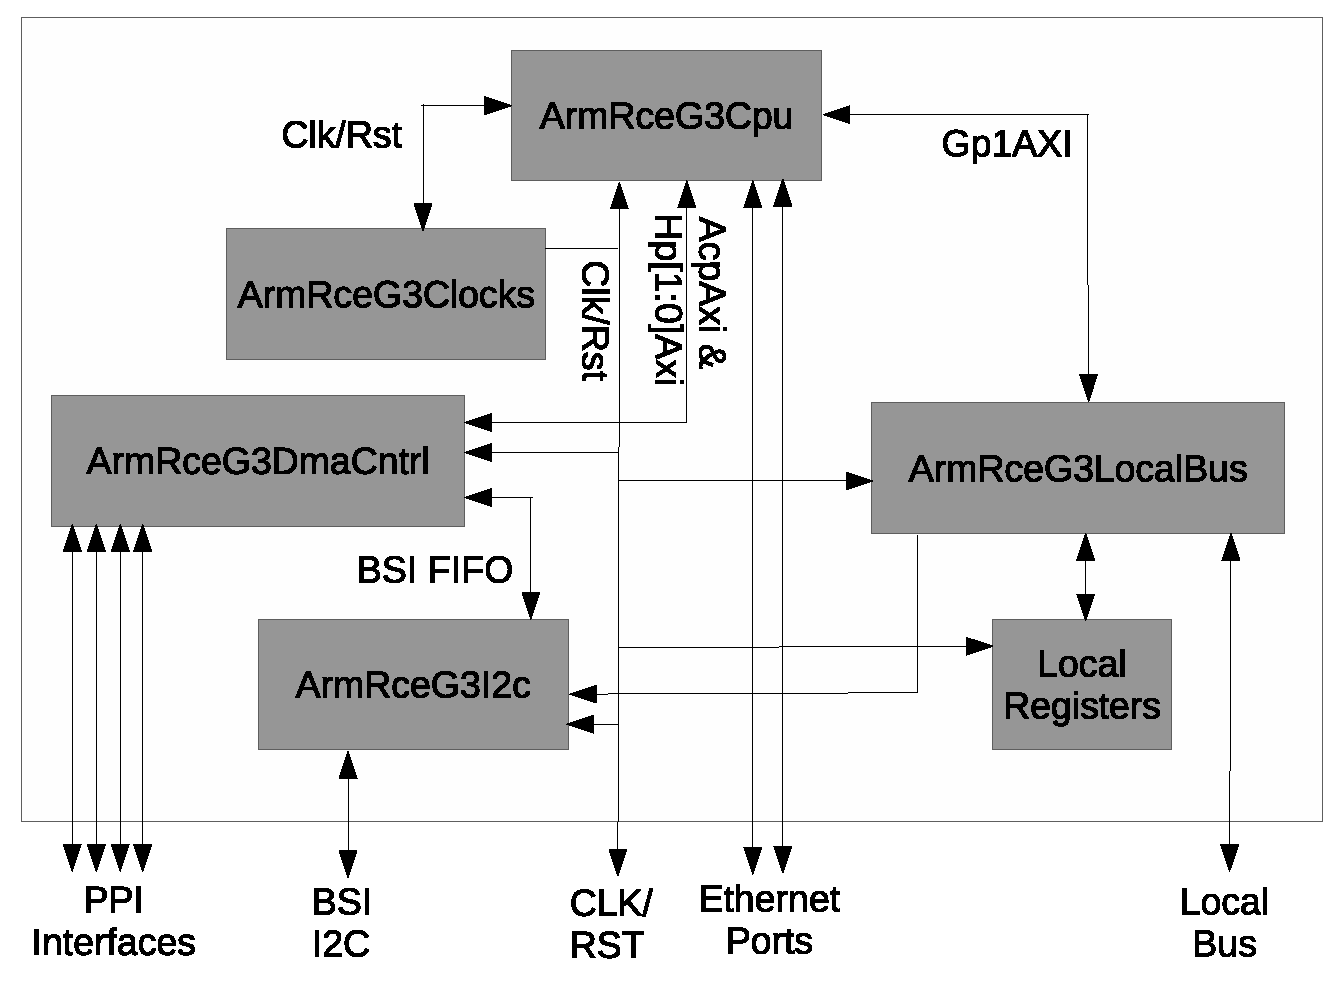
\psfig{file=images/arm_g3_top.eps,scale=0.50}
   \caption{Top Level Block Diagram}
   \label{fig:top_level_block}
\end{figure}


\subsection{Local AXI Controller (ArmRceG3LocalAxi.vhd)}
\label{subsec:ArmRceG3LocalAxi}

This module implements a bridge between the general purpose AXI master port (GP1) and a number of internal AXI-Lite busses.
The local AXI controller supports single dual word (32-bit) accesses.

\subsubsection{RCE Core Address Space}

The overall address map for the RCE core is shown in table \ref{tab:rce_core_map}. 

\begin{table}[H]
\small
\centering
   \begin{tabular}{| l | l | l | } 
      \hline \textbf{Address Range} & \textbf{Assignment} \\
      \hline 0x8000\_0000 - 0x8000\_FFFF & Top Level Registers \\
      \hline 0x8400\_0000 - 0x8400\_0FFF & BSI I2C Slave Registers \\
      \hline 0x8800\_0000 - 0x8800\_0FFF & DMA Controller Registers \\
      \hline 0x8800\_1000 - 0x8800\_10FF & DMA Controller Completion FIFOs \\
      \hline 0x8800\_1100 - 0x8800\_11FF & DMA Controller Free List FIFOs \\
      \hline 0xA000\_0000 - 0xBFFF\_FFFF & External Address Space \\
      \hline
   \end{tabular}
   \caption{RCE Core Address Space }
   \label{tab:rce_core_map}
\end{table}

\subsubsection{Top Level Address Map}

The local AXI controller module contains a handful of registers as shown in the following table. 

The Version value is unique to each target FPGA design. While the format of this version value is not defined it is typical for the upper 
12 bits to be unique for each target FPGA type while the lower 20 bits are incremented with each compile.

The ArmRceG3Version value is defined in the core module and is incremented any time any of the major functions within the core module are
modified.

The BuildString value is a 256 character NULL terminated string which contains information about the user who built the image and the 
timestamp of when the image was built. This field is automatically updated by the build script at each compile.

\begin{table}[H]
\small
\centering
   \begin{tabular}{| l | l | l | l | l | } 
      \hline \textbf{Address} & \textbf{Bits} & \textbf{Mode} & \textbf{Name} & \textbf{Description} \\
      \hline 0x80000000       & 31:0          & Read     & Version         & FPGA version value. Set in Version.vhd. \\
      \hline 0x80000004       & 31:0          & R/W      & Scratchpad      & Scratchpad register.                                 \\
      \hline 0x80000008       & 31:0          & Read     & ArmRceG3Version & ARM RCE Gen3 Module Version.                         \\
      \hline 0x80000010       & 1:0           & R/W      & ClkSel0         & Reference Clock 0 Frequency Select. \\               \\
      \hline 0x80000014       & 1:0           & R/W      & ClkSel1         & Reference Clock 1 Frequency Select. \\               \\
      \hline 0x80000020       & 31            & Read     & DNA Valid       & Device DMA value is valid.                           \\
                              & 23:0          & Read     & DNA Value 56:32 & Bits 56:32 of Xilinx device DNA value.               \\
      \hline 0x80000024       & 31:0          & Read     & DNA Vlaue 31:00 & bits 31:00 of Xilinx device DNA value.               \\
      \hline 0x80001000 - 0x800010FF & 31:0   & Read     & BuildString     & NULL termination build user and timestamp string.    \\
      \hline
   \end{tabular}
   \caption{Top Level Address Map}
   \label{tab:top_addr}
\end{table}

The AXI-Lite busses inside the RCE core module operate at 200Mhz while the external AXI-Lite bus operates at 125Mhz.

\subsection{Clock Generation Module (ArmRceG3Clocks.vhd)}
\label{subsec:ArmRceG3Clocks}

The clock generation module generates the set of clocks required both internal and external to
the ARM RCE Gen 3 Core module. The clocks in this module can be derived from any of the four function 
clock outputs from the processor core. Currently all clocks are derived from function clock 0 which is
required to be configured as 100Mhz.

The following clock and reset siganls are generated within the clock generation module.

\begin{table}[H]
\small
\centering
   \begin{tabular}{| l | l | l | l | l | } 
      \hline \textbf{Signal} & \textbf{Description} \\
      \hline dmaClk          & DMA AXI bus clock output, 200Mhz   \\
      \hline dmaClkRst       & DMA AXI bus clock reset            \\
      \hline sysClk125       & System 125Mhz clock                \\
      \hline sysClk125Rst    & System 125Mhz clock reset          \\
      \hline sysClk200       & System 200Mhz clock                \\
      \hline sysClk200Rst    & System 200Mhz clock reset          \\
      \hline
   \end{tabular}
   \caption{ArmRceG3Clocks Clocks}
   \label{tab:clk_gen_clocks}
\end{table}

\subsection{DMA Controller (ArmRceG3DmaCntrl.vhd)}
\label{subsec:ArmRceG3DmaCntrl}

The DMA controller module is a container for the logic modules which implement the protocol plug in (PPI) interfaces as well
as the BSI management interface. 

\subsubsection{DMA Controller Block Diagram}

The block diagram of the DMA controller module is shown in figure \ref{fig:dma_cntrl_block}. The following sub modules
exist within the module and are described in greater detail later in this document:

\begin{itemize}
   \item ArmRceG3IbCntrl: Container for inbound FIFO logic modules (section \ref{subsec:ArmRceG3IbCntrl})
   \item ArmRceG3IbPpi: Inbound PPI controller module (section \ref{subsec:ArmRceG3IbPpi})
   \item ArmRceG3ObCntrl: Container for outbound FIFO logic modules (section \ref{subsec:ArmRceG3ObCntrl})
   \item ArmRceG3ObPpi: Outbound PPI controller module (section \ref{subsec:ArmRceG3ObPpi})
   \item ArmRceG3DmaComp: DMA completion FIFO container module (section \ref{subsec:ArmRceG3DmaComp})
\end{itemize}

The DMA controller module also contains a number of local configuration and status registers. 

\begin{figure}[H]
   \centering
   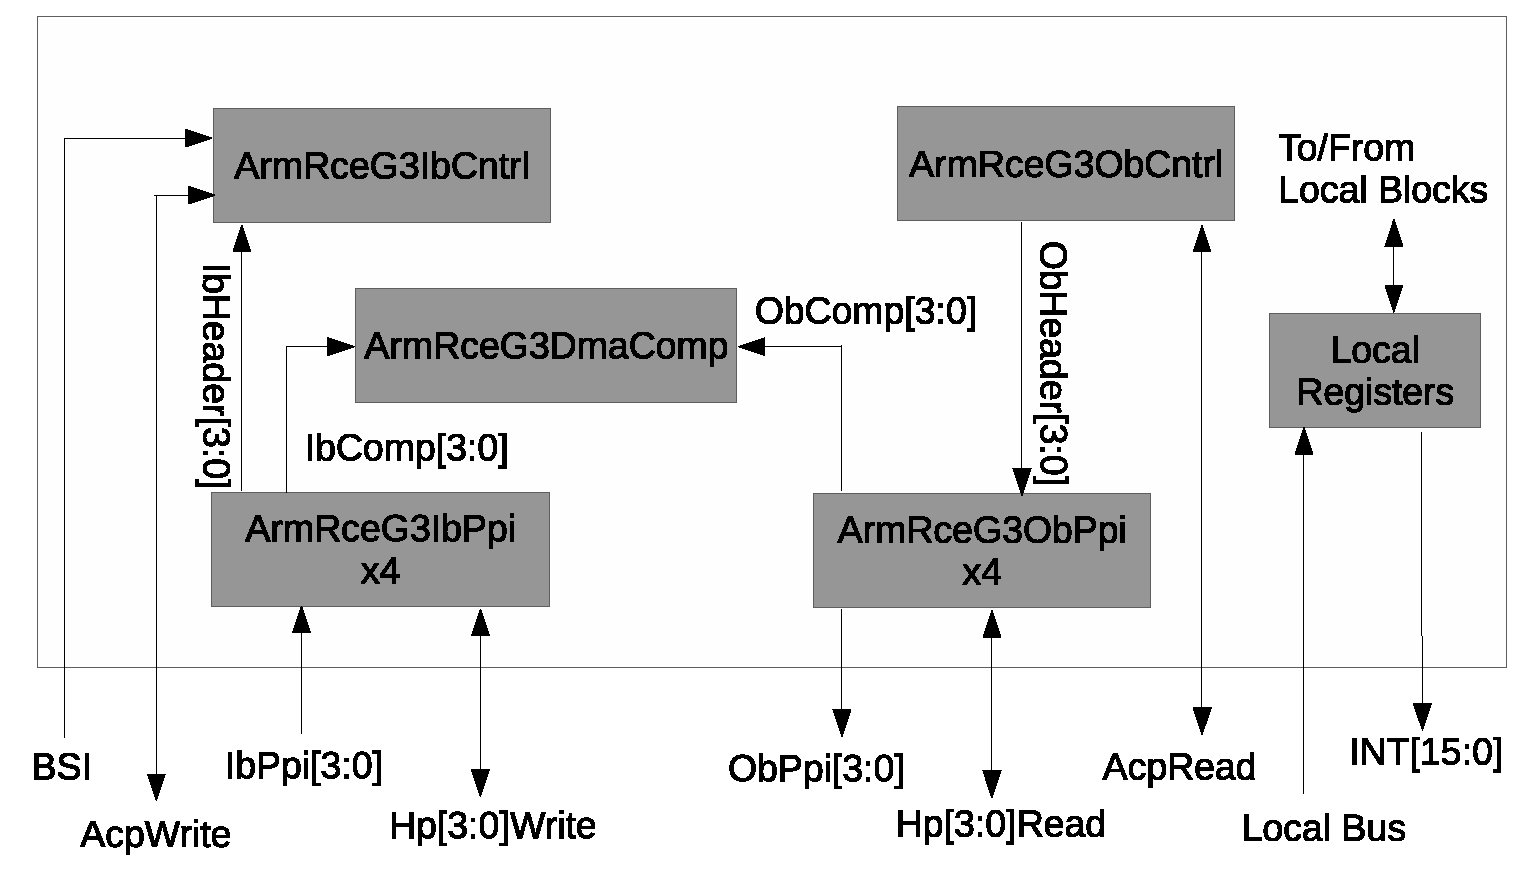
\psfig{file=images/arm_g3_dma_cntrl.eps,scale=0.50}
   \caption{DMA Controller Block Diagram}
   \label{fig:dma_cntrl_block}
\end{figure}

\subsubsection{DMA Controller Address Map}
The DMA controller module contains the register read/write logic for all of it's sub modules. The resulting address map is shown below.

\begin{center}[H]
\small
   \begin{longtable}{| l | l | l | l | l | }
      \hline \textbf{Address} & \textbf{Bits} & \textbf{Mode} & \textbf{Name}   & \textbf{Description} \\
      \hline
      \endfirsthead
      \multicolumn{5}{c}%
      {\textit{Continued from previous page}} \\
      \hline \textbf{Address} & \textbf{Bits} & \textbf{Mode} & \textbf{Name}   & \textbf{Description} \\
      \hline
      \endhead
      \hline \multicolumn{5}{r}{\textit{Continued on next page}} \\
      \endfoot
      \hline
      \caption{DMA Controller Address Map} \\
      \endlastfoot
      \hline 0x88000000 - 0x880000FC & NA    & Read  & Unused               & Read as zero                                   \\
      \hline 0x88000100 - 0x8800013C & 31:0  & Write & InboundHeader0Free   & Inbound header 0, free list FIFO               \\
                                     &       &       &                      & FIFO bits 35:32 = Address bits 5:2             \\
      \hline 0x88000140 - 0x8800017C & 31:0  & Write & InboundHeader1Free   & Inbound header 1, free list FIFO               \\
                                     &       &       &                      & FIFO bits 35:32 = Address bits 5:2             \\
      \hline 0x88000180 - 0x880001BC & 31:0  & Write & InboundHeader2Free   & Inbound header 2, free list FIFO               \\
                                     &       &       &                      & FIFO bits 35:32 = Address bits 5:2             \\
      \hline 0x880001C0 - 0x880001FC & 31:0  & Write & InboundHeader3Free   & Inbound header 3, free list FIFO               \\
                                     &       &       &                      & FIFO bits 35:32 = Address bits 5:2             \\
      \hline 0x88000200 - 0x8800023C & 31:0  & Write & OutboundHeader0Tx    & Outbound header 0, transmit FIFO               \\
                                     &       &       &                      & FIFO bits 35:32 = Address bits 5:2             \\
      \hline 0x88000240 - 0x8800027C & 31:0  & Write & OutboundHeader1Tx    & Outbound header 1, transmit FIFO               \\
                                     &       &       &                      & FIFO bits 35:32 = Address bits 5:2             \\
      \hline 0x88000280 - 0x880002BC & 31:0  & Write & OutboundHeader2Tx    & Outbound header 2, transmit FIFO               \\
                                     &       &       &                      & FIFO bits 35:32 = Address bits 5:2             \\
      \hline 0x880002C0 - 0x880002FC & 31:0  & Write & OutboundHeader3Tx    & Outbound header 3, transmit FIFO               \\
                                     &       &       &                      & FIFO bits 35:32 = Address bits 5:2             \\
      \hline 0x88000300              & NA    & Write & MemChan0DirtyClear   & Write to clear memory channel 0                \\
      \hline 0x88000304              & NA    & Write & MemChan1DirtyClear   & Write to clear memory channel 1                \\
             \ldots                  &       &       &                      &                                                \\
      \hline 0x88000310              & NA    & Write & MemChan4DirtyClear   & Write to clear memory channel 4                \\
      \hline 0x88000314 - 0x880003FC & NA    & Read  & Unused               & Read as zero                                   \\
      \hline 0x88000400              & 3:0   & Read  & IbDirtyStatus        & Inbound memory dirty, one bit per channel \\
                                     & 4     & Read  & BsiDirtyStatus       & BSI memory dirty, one bit per channel \\
                                     & 15:5  & Read  & CompFifoStatus       & Completion FIFO ready, one bit per channel \\
      \hline 0x88000404              & 15:0  & R/W   & InterruptEnable      & Interrupt enable, one bit per interrupt        \\
      \hline 0x88000408              & 3:0   & R/W   & HeaderWriteDmaCache  & Header AXI write cache configuration           \\
      \hline 0x8800040C              & 3:0   & R/W   & HeaderReadDmaCache   & Header AXI read cache configuration            \\
      \hline 0x88000410              & 3:0   & R/W   & IbFifoEnable         & Inbound header enables                         \\
                                     & 4     & R/W   & BsiFifoEnable        & BSI FIFO enable                                \\
                                     & 8:5   & R/W   & ObFifoEnable         & Outbound header enables                        \\
      \hline 0x88000418              & 31:18 & R/W   & MemBaseAddress       & Memory base address                            \\
      \hline 0x8800041C              & 3:0   & R/W   & PpiReadDmaCache      & PPI AXI read cache configuration               \\
      \hline 0x88000420              & 3:0   & R/W   & PpiWriteDmaCache     & PPI AXI write cache configuration              \\
      \hline 0x88000424              & 3:0   & R/W   & PpiIbOnline[3:0]     & Inbound PPI online configuration              \\
                                     & 7:4   & R/W   & PpiObOnline[3:0]     & Outbound PPI online configuration             \\
      \hline 0x88000428 - 0x880004FC & NA    & Read  & Unused               & Read as zero                                   \\
      \hline 0x88000500 - 0x8800053C & 31:0  & Write & InboundPpi0Control   & Inbound PPI 0 Control FIFO                     \\
                                     &       &       &                      & FIFO bits 35:32 = Address bits 5:2             \\
      \hline 0x88000540 - 0x8800057C & 31:0  & Write & InboundPpi1Control   & Inbound PPI 1 Control FIFO                     \\
                                     &       &       &                      & FIFO bits 35:32 = Address bits 5:2             \\
      \hline 0x88000580 - 0x880005BC & 31:0  & Write & InboundPpi2Control   & Inbound PPI 2 Control FIFO                     \\
                                     &       &       &                      & FIFO bits 35:32 = Address bits 5:2             \\
      \hline 0x880005C0 - 0x880005FC & 31:0  & Write & InboundPpi3Control   & Inbound PPI 3 Control FIFO                     \\
                                     &       &       &                      & FIFO bits 35:32 = Address bits 5:2             \\
      \hline 0x88000600              & 31:0  & Read  & IbPpi0Id             & Inbound PPI 0 ID value                         \\
      \hline 0x88000604              & 31:0  & Read  & IbPpi0Id             & Inbound PPI 0 version value                      \\
      \hline 0x88000608              & 31:0  & Read  & IbPpi0ConfigA        & Inbound PPI 0 config word A              \\
      \hline 0x8800060C              & 31:0  & Read  & IbPpi0ConfigB        & Inbound PPI 0 config word B              \\
             \ldots                  &       &       &                      &                                                \\
      \hline 0x88000630              & 31:0  & Read  & IbPpi3Id             & Inbound PPI 3 ID value                         \\
      \hline 0x88000634              & 31:0  & Read  & IbPpi3Id             & Inbound PPI 3 version value                      \\
      \hline 0x88000638              & 31:0  & Read  & IbPpi3ConfigA        & Inbound PPI 3 config word A              \\
      \hline 0x8800063C              & 31:0  & Read  & IbPpi3ConfigB        & Inbound PPI 3 config word B              \\
      \hline 0x88000640              & 31:0  & Read  & ObPpi0Id             & Outbound PPI 0 ID value                         \\
      \hline 0x88000644              & 31:0  & Read  & ObPpi0Id             & Outbound PPI 0 version value                      \\
      \hline 0x88000648              & 31:0  & Read  & ObPpi0ConfigA        & Outbound PPI 0 config word A              \\
      \hline 0x8800064C              & 31:0  & Read  & ObPpi0ConfigB        & Outbound PPI 0 config word B              \\
             \ldots                  &       &       &                      &                                                \\
      \hline 0x88000670              & 31:0  & Read  & ObPpi3Id             & Outbound PPI 3 ID value                         \\
      \hline 0x88000674              & 31:0  & Read  & ObPpi3Id             & Outbound PPI 3 version value                      \\
      \hline 0x88000678              & 31:0  & Read  & ObPpi3ConfigA        & Outbound PPI 3 config word A              \\
      \hline 0x8800067C              & 31:0  & Read  & ObPpi3ConfigB        & Outbound PPI 3 config word B              \\
      \hline 0x88000680 - 0x88000FFC & NA    & Read  & Unused               & Read as zero                                   \\
      \hline 0x88001000              & 31:0  & Read  & CompFifo0            & Completion FIFO 0                              \\
      \hline 0x88001004              & 31:0  & Read  & CompFifo1            & Completion FIFO 1                              \\
             \ldots                  &       &            &                      &                                                \\
      \hline 0x88001028              & 31:0  & Read  & CompFifo10           & Completion FIFO 10                             \\
      \hline 0x8800102C - 0x88001038 & NA    & Read  & Unused               & Read as zero                                   \\
      \hline 0x8800103C              & 31:0  & R/W   & CompFreeFifo         & Completion Free List FIFO                      \\
      \hline 0x88001040 - 0x880010FC & NA    & Read  & Unused               & Read as zero                                   \\
      \hline 0x88001100              & 31:0  & Read  & OutboundHeader0Free  & Outbound Header 0 Free List                    \\
      \hline 0x88001104              & 31:0  & Read  & OutboundHeader1Free  & Outbound Header 1 Free List                    \\
      \hline 0x88001108              & 31:0  & Read  & OutboundHeader2Free  & Outbound Header 2 Free List                    \\
      \hline 0x8800110C              & 31:0  & Read  & OutboundHeader3Free  & Outbound Header 3 Free List                    \\
      \hline 0x88001110 - 0x880011FC & NA    & Read  & Unused               & Read as zero                                   \\
      \hline
   \end{longtable}
   \label{tab:dma_addr}
\end{center}

A number of FIFOs in the above table are 36-bit FIFOs which are written to over the 32-bit local bus. The upper 4 bits of the FIFO are derived by 
the offset address used when writing to the FIFO. The address for the FIFO write can be derived using the following
equation:

\begin{center}
Address = (FIFO base address) * 4 * (Bits 35:32)
\end{center}

For example to write the value 0xA\_5A5A\_5A5A to the Inbound header 0 free list FIFO, one 
would write the 32-bit value 0x5A5A\_5A5A to the address 0x8800\_0128.

\subsubsection{DMA Controller Interrupt Mapping}

The DMA controller supports 16 interrupt putputs, each with it's own enable bit. The sources of these 16 interrupts are described in the table below.

\begin{table}[H]
\small
\centering
   \begin{tabular}{| l | l | l | }
      \hline \textbf{Interrupt} & \textbf{Name}  & \textbf{Description} \\
      \hline 3:0            & IbDesc[3:0]    &  Inbound header 3:0 descriptor FIFOs. \\
                            &                &  Asserted when associated quad word memory location \\
                            &                &  is dirty. De-asserted when the associated memory location \\
                            &                &  is cleaned by writing to corresponding dirty clear address. \\
      \hline 4              & BsiData        &  BSI data FIFO.                      \\
                            &                &  Asserted when associated quad word memory location \\
                            &                &  is dirty. De-asserted when the associated memory location \\
                            &                &  is cleaned by writing to corresponding dirty clear address. \\
      \hline 15:5           & CompFifo[10:0] &  Completion FIFOs.                   \\
                            &                &  Asserted when associated completion FIFO has at least one entry. \\
                            &                &  De-asserted when the associated completion FIFO is empty. \\
      \hline
   \end{tabular}
   \caption{DMA Controller Interrupt Mapping}
   \label{tab:dma_int_mappings}
\end{table}

\subsection{Inbound Controller (ArmRceG3IbCntrl.vhd)}
\label{subsec:ArmRceG3IbCntrl}

The inbound controller module is a sub-container within the DMA controller which contains the logic to support inbound PPI traffic. 
This includes the 4 inbound header engines, the 5 quad word FIFOs, the memory space dirty state tracking logic and an AXI write controller.
The AXI write controller is the interface between the various write engines and the write interface of the AXI ACP processor bus. 

\subsubsection{Inbound Controller Block Diagram}

The block diagram of the inbound controller module is shown in figure \ref{fig:ib_cntrl_block}. The following sub modules
exist within the module and are described in greater detail later in this document:

\begin{itemize}
   \item ArmRceG3IbHeaderFifo: Inbound header transfer FIFO and control logic (section \ref{subsec:ArmRceG3IbHeaderFifo})
   \item ArmRceG3IbQWordFifo: Inbound Quad Word FIFO and control logic (section \ref{subsec:ArmRceG3IbQWordFifo})
   \item ArmRceG3AxiWriteCntrl: AXI write controller (section \ref{subsec:ArmRceG3AxiWriteCntrl})
\end{itemize}

The inbound controller module also contains dirty status logic which tracks the state of the OCM memory locations associated
with the 5 quad word FIFO modules.


\begin{figure}[H]
   \centering
   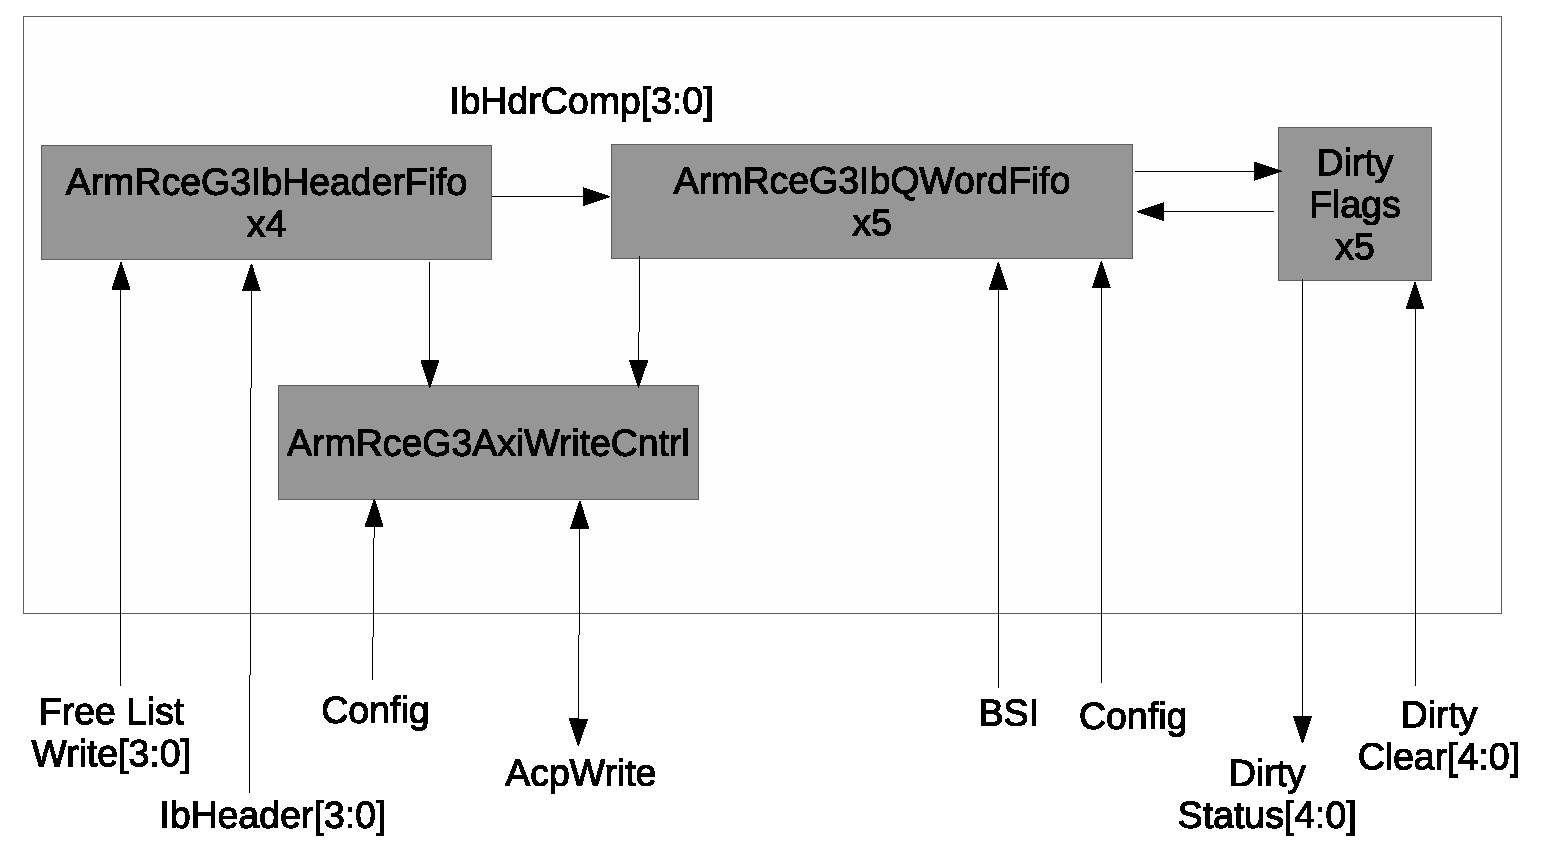
\psfig{file=images/arm_g3_ib_cntrl.eps,scale=0.50}
   \caption{Inbound Controller Block Diagram}
   \label{fig:ib_cntrl_block}
\end{figure}

\subsubsection{Quad Word FIFO Channels}

The inbound controller contains 5 instances of the Quad Word FIFO module described in section \ref{subsec:ArmRceG3IbQWordFifo}. The assignment and destination
memory address of each of these instances is shown in table \ref{tab:ib_qword_mappings}.

\begin{table}[H]
\small
\centering
   \begin{tabular}{| l | l | l | l | }
      \hline \textbf{Index} & \textbf{Name}  & \textbf{Destination Address} & \textbf{Description} \\
      \hline 0              & IbDesc0        & memBaseAddress + 0x00 &  Inbound header 0 descriptor FIFO \\
      \hline 1              & IbDesc1        & memBaseAddress + 0x08 &  Inbound header 1 descriptor FIFO \\
      \hline 2              & IbDesc2        & memBaseAddress + 0x10 &  Inbound header 2 descriptor FIFO \\
      \hline 3              & IbDesc3        & memBaseAddress + 0x18 &  Inbound header 3 descriptor FIFO \\
      \hline 4              & BsiData        & memBaseAddress + 0x20 &  BSI data FIFO                       \\
      \hline
   \end{tabular}
   \caption{Quad Word FIFO Channels}
   \label{tab:ib_qword_mappings}
\end{table}

The four inbound header descriptor FIFOs are populated when the inbound header engine (see section \ref{subsec:ArmRceG3IbHeaderFifo})
completes a header transfer. The BSI data FIFO is populated when the IPMI controller writes a 32-bit word to the
BSI shared memory over the management I2C bus (see section \ref{subsec:ArmRceG3I2c}). 

\subsubsection{ACP Write ID Mapping}

The ACP AXI interface only supports 8 independent transaction IDs. Since the inbound controller contains 5 potentional masters, some
IDs need to be shared. Table \ref{tab:ib_id_mappings} shows the allocation of AXI IDs to the masters within the inbound
controller. Only one master assigned to an ID can have an outstanding write transactions at any given time. Any other
masters which share an ID with a master who has an outstanding transaction will not attempt to access the ACP bus
until the outstanding transaction completes.

\begin{table}[H]
\small
\centering
   \begin{tabular}{| l | l | l |}
      \hline \textbf{AXI ID} & \textbf{FIFO(s)}      & \textbf{Function(s)}    \\
      \hline 0               & IbHeaderFifo0         & Inbound header 0 engine \\
      \hline 1               & IbHeaderFifo1         & Inbound header 1 engine \\
      \hline 2               & IbHeaderFifo2         & Inbound header 2 engine \\
      \hline 3               & IbHeaderFifo3         & Inbound header 3 engine \\
      \hline 4               & QWordFifo0            & Inbound header 0 descriptor FIFO    \\
                             & QWordFifo4            & BSI FIFO                \\
      \hline 5               & QWordFifo1            & Inbound header 1 descriptor FIFO   \\
      \hline 6               & QWordFifo2            & Inbound header 2 descriptor FIFO   \\
      \hline 7               & QWordFifo3            & Inbound header 3 descriptor FIFO   \\
      \hline
   \end{tabular}
   \caption{ACP Write ID Mapping}
   \label{tab:ib_id_mappings}
\end{table}

\subsection{Quad Word FIFO Controller (ArmRceG3IbQWordFifo.vhd)}
\label{subsec:ArmRceG3IbQWordFifo}

The quad word FIFO controller is a block of logic which serves as a 63-bit FIFO with direct access to the on chip memory (OCM) contained within the 
Zynq processor. Only 63 bits are available because the upper bit is used for handshaking between the quad word FIFO module and the software 
driver. 

When an entry is available in the FIFO, the transfer state machine will check to see if the associated OCM memory space
is clearn or dirty as indicated by the 5-bit dirty vector managed by the indbound controller module. If the associated memory location 
is clean the transfer state machine will pull the 63-bit value from the FIFO and write it to the associated OCM memory location. Bit 64
of the memory location will be set to zero to indicate that the location has been updated.

All transactions generated by the quad word FIFO controller are a single 64-bit write transaction on the ACP bus. Once the write data portion
of the transaction is completed the transfer state machine will release the AXI bus. The associated AXI ID will be marked busy while the state 
machine waits for the write transaction to be acknowledged by the AXI bus.  When the write has completed the transfer state machine will clear 
the ID busy signal, mark the memory location as dirty and return to the idle state. 

If enabled the dirty flag of the memory location will trigger a processor interrupt. Some time later, after accessing the associated memory location 
in OCM, software will clean the memory location by performing a write access to the associated address space. The transfer state machine will
then transfer the next FIFO entry when available.

The FIFO logic will not operated until its associated fifoEnable signal is set via register access.

\subsubsection{Quad Word FIFO Block Diagram}

The quad word FIFO module consists of a 72-bit wide by 512 entry deep input FIFO and a transfer state machine.

\begin{figure}[H]
   \centering
   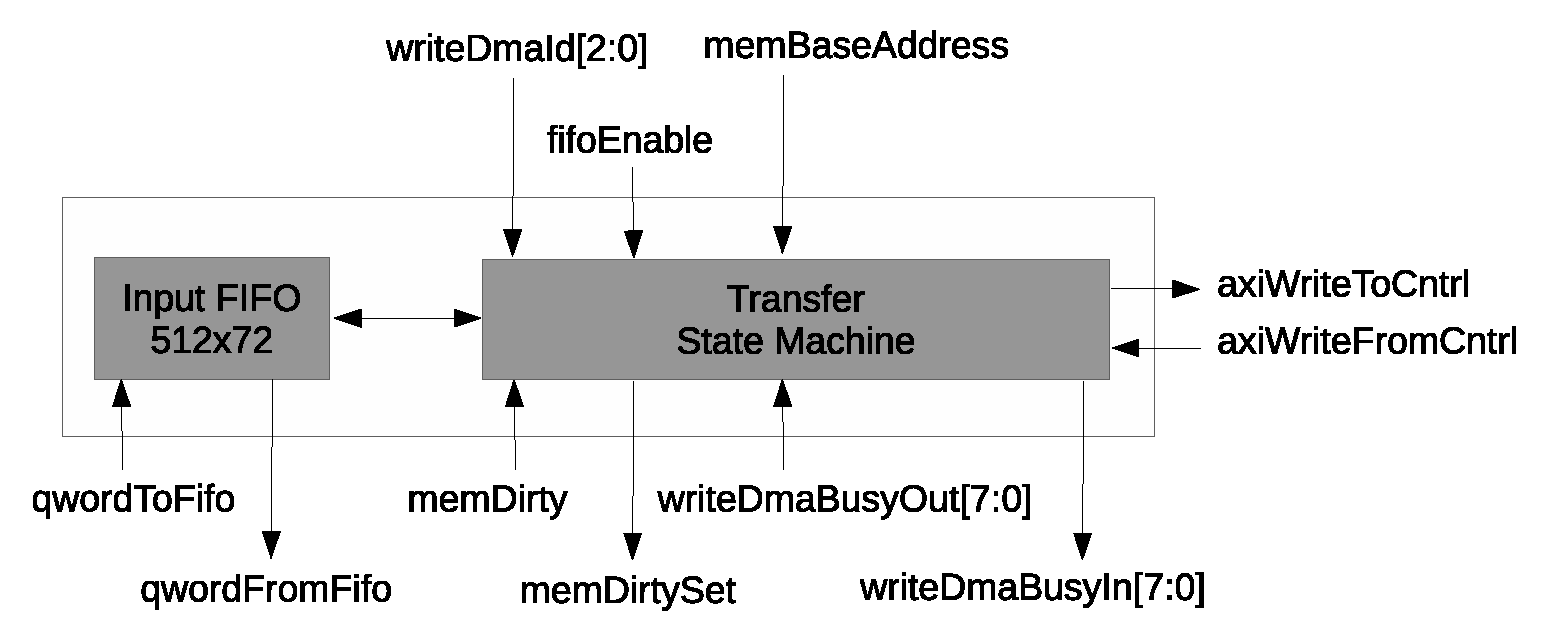
\psfig{file=images/arm_g3_qw_fifo.eps,scale=0.50}
   \caption{Quad Word FIFO Block Diagram}
   \label{fig:qw_fifo_block}
\end{figure}

\subsection{Inbound Header FIFO (ArmRceG3IbHeaderFifo.vhd)}
\label{subsec:ArmRceG3IbHeaderFifo}

The function of the inbound header FIFO module is to receive a PPI header and transfer it into on chip memory (OCM). 

When data is available in the FIFO the transfer engine will exit the idle state and pull a free descriptor entry
from the free list FIFO. The write address vector within the transfer engine is then preset with the sum of the
memBaseAddress and offset address contained in the descriptor. The offset value in the descriptor must be aligned to 
a cache line boundary.

Each AXI bus transaction originated by the transfer engine is a fixed size containing 32 bytes of data. 
The transfer engine will wait until a 32-byte block of data is ready in the FIFO or the end
of header (EOH) signal is detected. The transfer engine will request and release access to the AXI bus for each 32 byte
write transaction. If the EOH is in a position short of the 32 byte boundary, the transfer engine will continue to write
undefined data past the EOH location to the OCM.

When the entire frame has been transfered (as indicated by the EOH flag) the transfer engine will 
wait for all of the outstanding writes to complete. The transfer engine will then form a receive descriptor and 
write it to the associated inbound descriptor quad word FIFO. Along with the header length the type and mgmt flags 
from the received frame are included in the receive descriptor along with the error flag.

The inbound header FIFO will not operate if the associated fifoEnable configuration bit is not set.

\subsubsection{Inbound Header FIFO Block Diagram}

The inbound header FIFO module consists of a 72-bit wide by 512 entry deep input FIFO and a transfer state machine. A 36-bit x 512 entry FIFO is used
for the inbound free list. 

\begin{figure}[H]
   \centering
   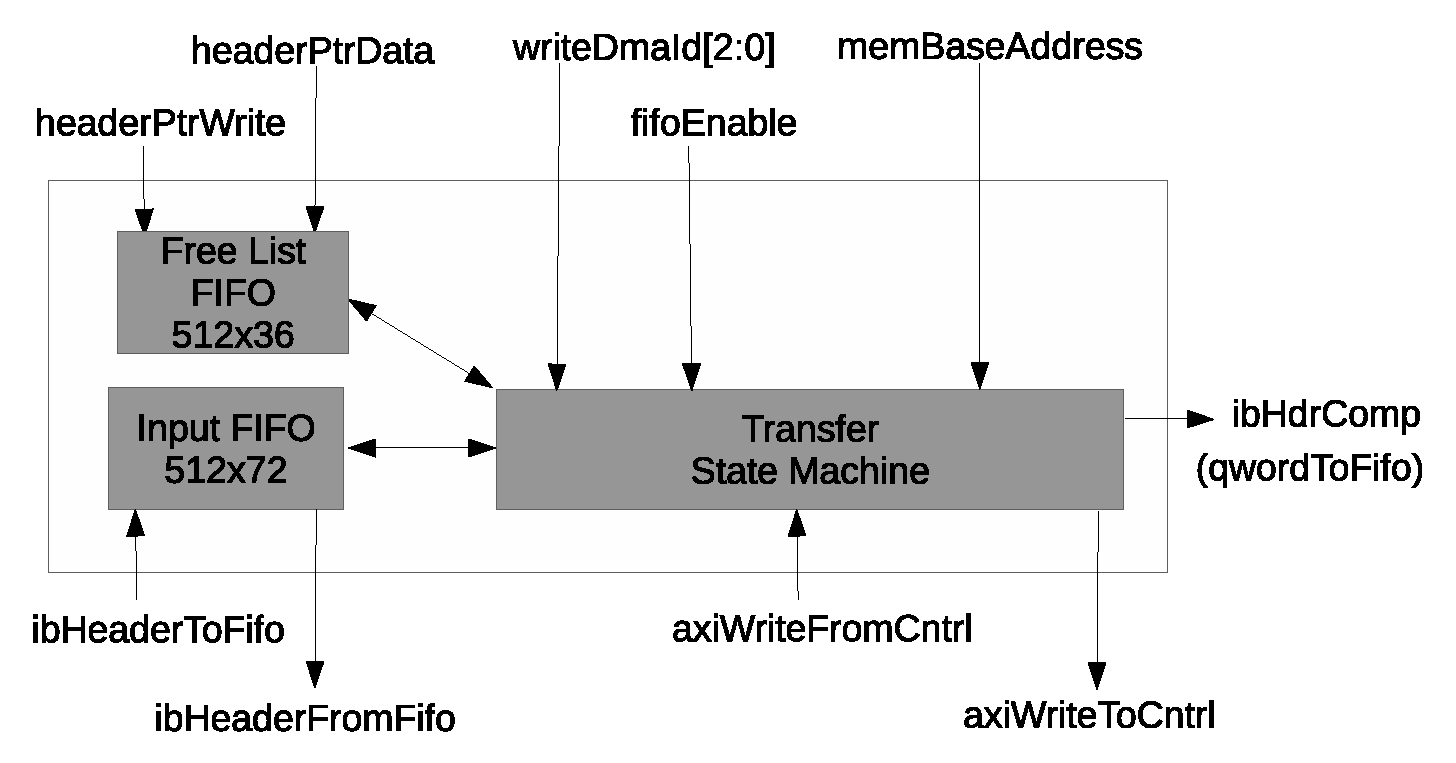
\psfig{file=images/arm_g3_ib_head_block.eps,scale=0.50}
   \caption{Inbound Header FIFO Block Diagram}
   \label{fig:ib_head_block}
\end{figure}

\subsubsection{Inbound Header Free List}

The inbound header free list contains a pool of memory address to which incoming headers are to be transfered.
This free list is populated by writing the allocated buffer address to the appropriate register address.
Since the upper data bits (35:32) of the free list FIFOs are not used only the base address for each FIFO is utilized. 
Each free list FIFO is capable of holding 511 free list entries.

The format of the receive free list entry is shown in table \ref{tab:ib_rx_flist}.

\begin{table}[H]
\small
\centering
   \begin{tabular}{| l | l | l | } 
      \hline \textbf{Bits} & \textbf{Name} & \textbf{Description} \\
      \hline 35:19         & unused        & ignored \\
      \hline 17:3          & address       & This field contains the offset address to which the inbound frame \\
                           &               & will be transfered. This address is relative to the configured base address  \\
                           &               & and must be cache line aligned.                                              \\
      \hline 2:0           & address       & Unused. The lower three address bits are assumed to be zero.               \\
      \hline
   \end{tabular}
   \caption{Inbound Header Free List Entry}
   \label{tab:ib_rx_flist}
\end{table}

\subsubsection{Inbound Header Receive Descriptor}

When an inbound header is received the inbound header logic will pull an address from the free list and DMA the header data to the associated address. 
When the operation has completed a receive descriptor will be placed in the associated receive queue. 
The receive queue is implemented in a \hyperref[subsec:ArmRceG3IbQWordFifo]{Quad Word FIFO} described in section \ref{subsec:ArmRceG3IbQWordFifo}. 
The mapping of the quad word FIFOs are described in section \ref{subsec:ArmRceG3IbCntrl}.

The format of the receive queue descriptor is shown in table \ref{tab:ib_rx_desc}.

\begin{table}[H]
\small
\centering
   \begin{tabular}{| l | l | l | } 
      \hline \textbf{Bits} & \textbf{Name} & \textbf{Description} \\
      \hline 63            & handshake     & Set to zero by firmware when valid     \\
      \hline 62:61         & unused        & Always zero                                                            \\ 
      \hline 60            & error         & This bit is set when the error bit was set on the inbound header.      \\
                           &               & This state is only possible when the inbound PPI frame has no payload. \\
      \hline 59:52         & unused        & Always zero                                                       \\
      \hline 51:48         & htype         & frame type field from inbound frame                                    \\
      \hline 47:40         & unused        & Always zero                                                       \\
      \hline 39:32         & length        & Length of received header. One based length (1=1, 2=2)                 \\
                           &               & Specified in number of 64-bit quad words transfered.                   \\
      \hline 31:18         & unused        & Always zero                                                       \\
      \hline 17:3          & address       & This field contains the offset address to which the inbound frame \\
                           &               & was transfered. This address is relative to the configured base address \\
                           &               & and must be cache line aligned.                                         \\
      \hline 2:0           & address       & These bits are always zero.                                                \\
      \hline
   \end{tabular}
   \caption{Inbound Header Receive Descriptor}
   \label{tab:ib_rx_desc}
\end{table}

\subsubsection{Inbound Header Flow Control}

The inbound header module asserts three flow control signals depending on the state of the input FIFO:

\begin{itemize}
  \item Full           = The FIFO is full, no free entries available.
  \item Almost Full    = The FIFO is almost full with one free entry left.
  \item Partially Full = The FIFO has less than 255 entries (out of 512) available.
\end{itemize}

\subsection{Inbound PPI Controller (ArmRceG3IbPpi.vhd)}
\label{subsec:ArmRceG3IbPpi}

The inbound PPI controller receives a complete PPI frame and separates the header from the payload. The header portion of the frame is forwarded  
to the associated inbound header controller module. Meanwhile payload portion of the frame is stored in a local FIFO. The internal state machine will
wait until a inbound PPI descriptor is available in the PPI control FIFO. This descriptor described in table \ref{tab:ib_ppi_cntrl} contains
the information needed to transfer the PPI frame into processor memory. When the inbound DMA operation has completed, a completion descriptor
is written to a targeted completion FIFO. The contents of this completion descriptor are detailed in table \ref{tab:ib_ppi_comp}.

Each inbound PPI engine is attached to one of the four HP AXI write interfaces. This dedicated connection means that the inbound PPI engine
can assume complete ownership of the interface. A simplified version of the AXI write controller (described in section \ref{subsec:ArmRceG3AxiWriteCntrl})
is instantiated in the module in order to simplify the state machine and improve timing performance. In order to ensure AXI bus efficiency all write 
transfers are a fixed size of 128 bytes. The write enable strobes are used to insure that only relevant payload data is written to memory and that the
transfer never exceeds the maximum frame size as indicated by the receive control descriptor.  

A byte realignment block is used to allow byte aligned transfer sizes and start addresses. The transfer size of the initial write block at the start 
of a new payload frame is adjusted in order to align the remaining transfers to 128 byte memory boundaries. This is done to ensure that none of the write 
transfers cross a 4-KByte boundary.

The inbound PPI engine does not have a mechanism to indicate errors on the incoming payload frame. If the PPI client indicates an error by asserting the ERR flag 
coincident with EOF or if the inbound payload frame overruns the allocated space, the error state is not communicated to the software layer.

\subsubsection{Inbound PPI Controller Block Diagram}

The inbound PPI controller module consists of a header receive engine which separates the incoming PPI frame into header and payload portions. The payload
portion of the frame is stored in a 72-bit wide by 512 deep payload FIFO. Receive descriptors are buffered in 36-bit by 512 entry FIFO. A transfer 
state machine controls the transfer of the input FIFO data to the Arm processor memory space. An ArmRceG3AxiWriteCntrl (see section \ref{subsec:ArmRceG3AxiWriteCntrl})
block serves as the bridge between the transfer state machine and the HP AXI bus. A 36-bit by 16 entry FIFO serves as a staging FIFO for completion records. 

\begin{figure}[H]
   \centering
   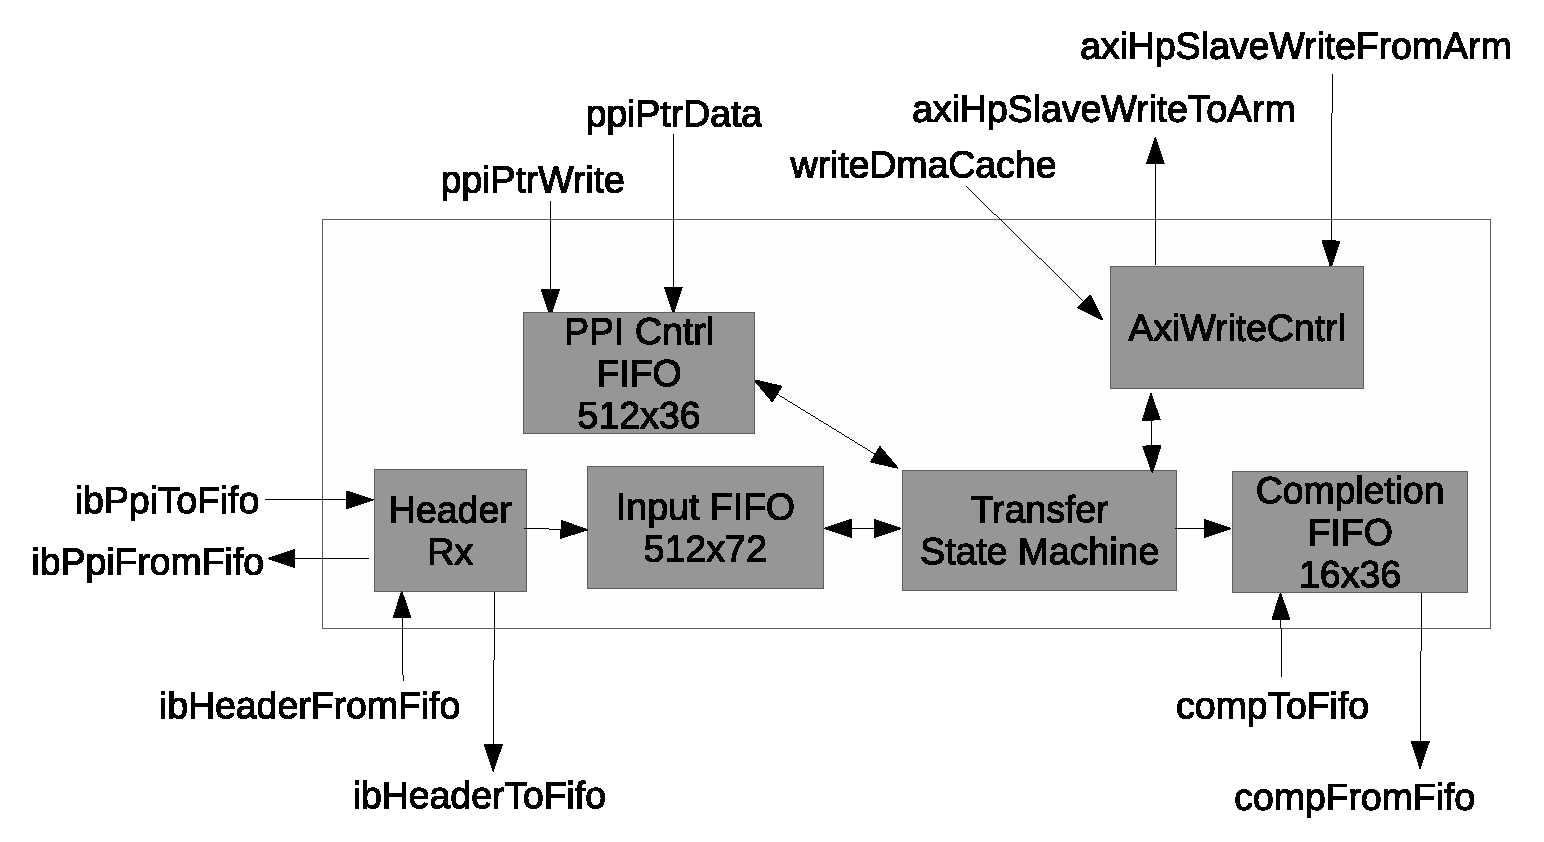
\psfig{file=images/arm_g3_ib_ppi.eps,scale=0.50}
   \caption{Inbound PPI Controller Block Diagram}
   \label{fig:ib_ppi_block}
\end{figure}

\subsubsection{Inbound PPI Receive Control}

When software wishes to initiate the reception of an inbound PPI payload it will write a receive control
descriptor to the inbound PPI control FIFO. The receive control descriptor requires three separate 
writes to the associated FIFO. Bits 35:32 of the FIFO entry are generated by adjusting offset address 
within the FIFO address space.

The format of the inbound PPI receive control descriptor is shown in table \ref{tab:ib_ppi_cntrl}.

\begin{table}[H]
\small
\centering
   \begin{tabular}{| l | l | l | l | l | l | } 
      \hline \textbf{DWord} & \textbf{Bits} & \textbf{Name} & \textbf{Description} \\
      \hline 0              & 35:33         & unused        & ignored                           \\
      \hline 0              & 32            & IbDrop        & Set this bit to discard frame     \\
      \hline 0              & 31:0          & IbAddr        & Inbound frame destination address \\
      \hline 1              & 35:33         & unused        & ignored                           \\
      \hline 1              & 32            & CompEn        & Set this bit to enable completion record generation \\
      \hline 1              & 31:0          & Length        & Length of inbound frame in bytes. \\
      \hline 2              & 35:32         & CompIndex     & Completion FIFO selection index.  \\
                            &               &               & Valid values are 0 - 10.          \\
      \hline 2              & 31:4          & CompId        & Id value for completion record    \\
      \hline
   \end{tabular}
   \caption{Inbound PPI Receive Descriptor}
   \label{tab:ib_ppi_cntrl}
\end{table}

\subsubsection{Inbound PPI Receive Completion Record}

When the inbound frame DMA operation is completed, the inbound PPI engine has the ability to add a completion record to one of the 11 
completion FIFOs. The CompEn bit in the inbound receive control descriptor determines if a completion record is 
generated and the CompIndex field determines which of the 11 FIFOs to route the completion record to. The value written 
to the completion record is defined in the CompId field of the inbound receive control record. When the IbDrop bit is set
a completion record is not generated.

The format of the receive completion record is shown in table \ref{tab:ib_ppi_comp}.

\begin{table}[H]
\small
\centering
   \begin{tabular}{| l | l | l | l | l | } 
      \hline \textbf{Bits} & \textbf{Name} & \textbf{Description} \\
      \hline 31:4          & CompId        & Completion ID field from receive descriptor.                           \\
      \hline 3             & User Error    & The PPI block asserted the error signals on the received frame.        \\
      \hline 2             & Length Error  & The incoming frame length did not match the receive descriptor.        \\
      \hline 1             & AXI Error     & An AXI write error occured.        \\
      \hline 0             & Invalid       & Asserted when the completion value is emtpy upon read. \\
      \hline
   \end{tabular}
   \caption{Inbound PPI Receive Completion Descriptor}
   \label{tab:ib_ppi_comp}
\end{table}

\subsubsection{Inbound PPI Flow Control}

The inbound PPI module will assert the pause signal to the PPI client firmware when the inbound frame FIFO has less than 255 entries (out of 512)
available. The pause signal will also be asserted when the associated inbound header FIFO also has less than 255 entires (out of 512) available.

\subsection{AXI Write Controller (ArmRceG3AxiWriteCntrl.vhd)}
\label{subsec:ArmRceG3AxiWriteCntrl}

The AXI write control module serves two purposes. The first is to provide arbitration between AXI masters in cases
where more than one write source is attached to a shared AXI bus. The second is to provide address and data FIFOs 
between the attached write state machine and the processor's AXI interface. This simplifies the implementation of the 
attached state machine and decouples the AXI interface flow control handshaking from the bursting nature of the 
attached write state machines.

The AXI write controller supports two modes of operation. The first supports 9 separate write masters when
used in the inbound controller block (see section \ref{subsec:ArmRceG3IbCntrl}). The second supports a single 
master when used in the in the inbound PPI controller (see section \ref{subsec:ArmRceG3IbPpi}).
When only master is attached the arbitration stage is optimized away to reduce latency.

\subsubsection{Axi Write Controller Block Diagram}

The AXI write controller contains an arbitration block which selects between one of 9 possible AXI masters. Address data and write data
are buffered in separate 36-bit x 512 entry FIFOs. Address and data engines convert the address and data FIFO entries into transactions on the AXI bus.

\begin{figure}[H]
   \centering
   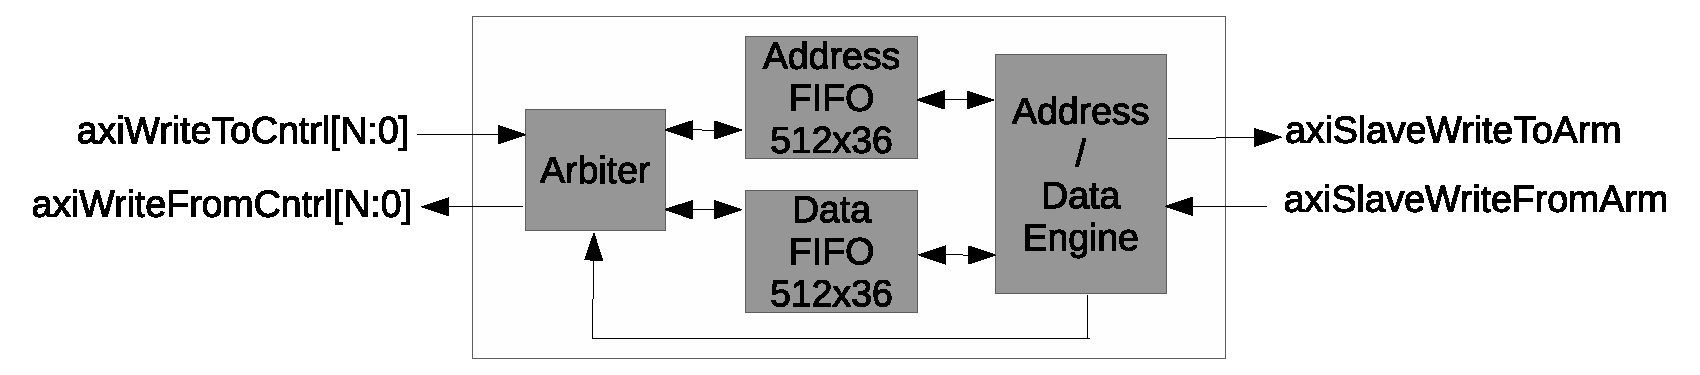
\psfig{file=images/arm_g3_axi_write.eps,scale=0.50}
   \caption{Axi Write Controller Block Diagram}
   \label{fig:axi_write_block}
\end{figure}

\subsection{Outbound Controller (ArmRceG3ObCntrl.vhd)}
\label{subsec:ArmRceG3ObCntrl}

The outbound controller module is a wrapper that contains four instances of the outbound header FIFO block and a single
instances of the AXI read control block. 

\subsubsection{Outbound Controller Block Diagram}

The block diagram of the outbound controller module is shown in figure \ref{fig:ob_cntrl_block}. The following sub modules
exist within the module and are described in greater detail later in this document:

\begin{itemize}
   \item ArmRceG3ObHeaderFifo: Inbound header transfer FIFO and control logic (section \ref{subsec:ArmRceG3IbHeaderFifo})
   \item ArmRceG3AxiReadCntrl: AXI write controller (section \ref{subsec:ArmRceG3AxiWriteCntrl})
\end{itemize}

The outbound controller module also contains 4 outbound free list FIFOs.

\begin{figure}[H]
   \centering
   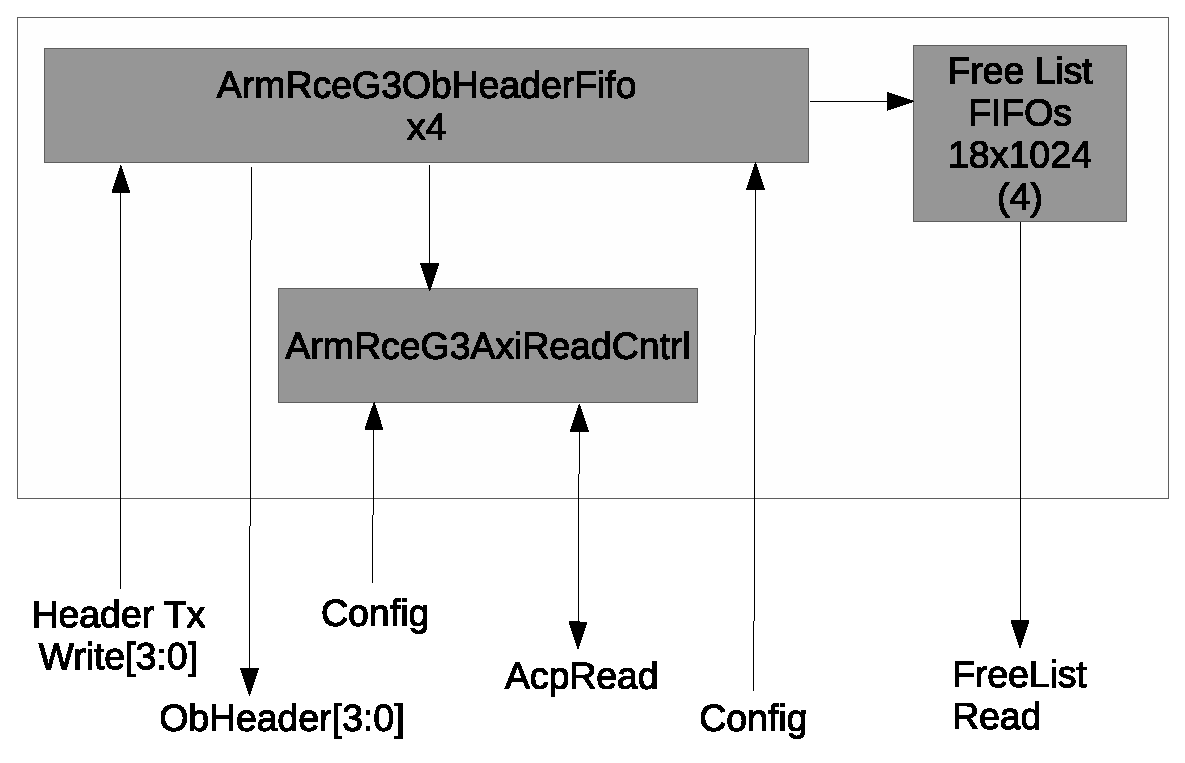
\psfig{file=images/arm_g3_ob_cntrl.eps,scale=0.50}
   \caption{Outbound Controller Block Diagram}
   \label{fig:ob_cntrl_block}
\end{figure}

\subsection{Outbound Header FIFO (ArmRceG3ObHeaderFifo.vhd)}
\label{subsec:ArmRceG3ObHeaderFifo}

The function of the outbound header FIFO module is to transfer PPI header data from OCM to the outbound PPI
module (see section \ref{subsec:ArmRceG3ObPpi}).

The transfer is started when software writes a transmit descriptor to the transmit list FIFO. The transfer state
machine will then exit the idle state, pull the offset address and length from the transmit descriptor and begin reading
from the OCM. Each read request is a fixed size of 32-bytes of data regardless of the length. The outbound 
transfer state machine will queue as many read requests as it has space left in it's outbound FIFO. Anytime the
transfer engine pauses for flow control it will release control of the AXI bus allowing it to be re-arbitrated. 

When the transmission operation is complete the offset address from the transmit descriptor will be placed back
on the free list.

The outbound header FIFO will not operate if the associated fifoEnable configuration bit is not set.

\subsubsection{Outbound Header FIFO Block Diagram}

The outbound header FIFO module consists of a 72-bit wide by 512 entry deep input FIFO and a transfer state machine. A 36-bit x 512 entry FIFO is used
for outbound transmit control.

\begin{figure}[H]
   \centering
   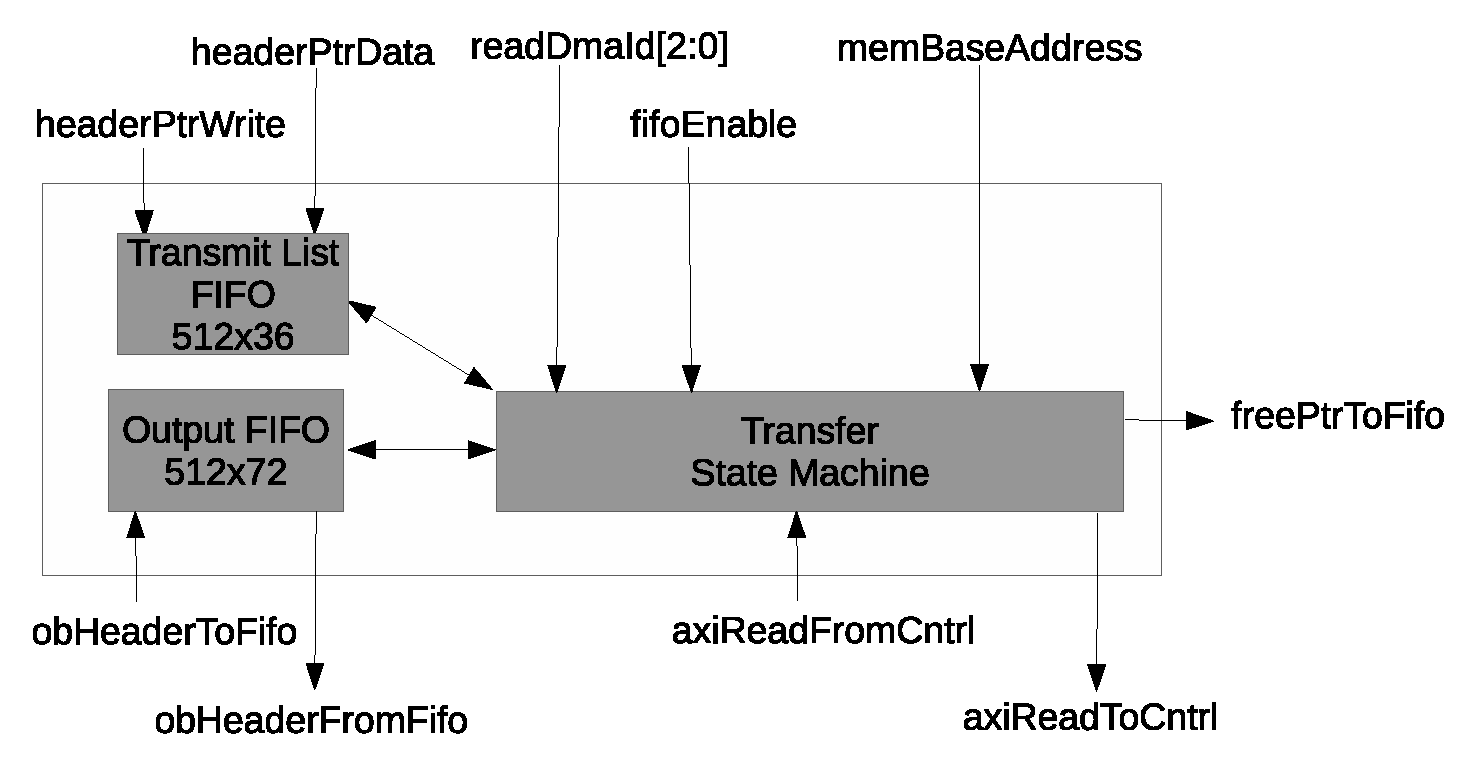
\psfig{file=images/arm_g3_ob_head_block.eps,scale=0.50}
   \caption{Outbound Header FIFO Block Diagram}
   \label{fig:ob_head_block}
\end{figure}

\subsubsection{Outbound Header Free List}

Each of the outbound header FIFOs provide a descriptor free list.  This free list is implemented in a local FIFO which is read over the local bus. 
At startup the software will populate the free list by submitting transmit descriptors with the transfer bit set (described in section \ref{subsec:ob_tx_desc}). 
During normal operation the software will pull a free transmit buffer from the free list and provide it to the header engine as part of the transmit descriptor. 
When the transmit operation has completed the address will be returned to the free list. 

The format of the outbound free list entry is shown in table \ref{tab:ob_tx_flist}.

\begin{table}[H]
\small
\centering
   \begin{tabular}{| l | l | l | l | l | } 
      \hline \textbf{Bits} & \textbf{Name} & \textbf{Description} \\
      \hline 31            & valid         & Bit to indicate if read entry is valid. \\
      \hline 30:18         & unused        & Read as zero.                                                        \\
      \hline 17:3          & address       & This field contains the offset address for the outbound header    \\
                           &               & free list. This address is relative to the configured base address \\
                           &               & and must be cache line aligned.                                    \\
      \hline 2:0           & address       & These bits are always zero.                                                \\
      \hline
   \end{tabular}
   \caption{Outbound Header Free List Entry}
   \label{tab:ob_tx_flist}
\end{table}

\subsubsection{Outbound Header Transmit Descriptor}
\label{subsec:ob_tx_desc}

An outbound header transmission is started by writing a descriptor to the appropriate header transmit FIFO. 
Since the upper data bits (35:32) of the transmit FIFOs are not used only the base address per each FIFO is utilized. 
Each transmit FIFO is capable of holding 511 free list entries. 
The format of the transmit header descriptor is shown in table \ref{tab:ob_tx_desc}.

\begin{table}[H]
\small
\centering
   \begin{tabular}{| l | l | l | l | l | } 
      \hline \textbf{Bits} & \textbf{Name} & \textbf{Description} \\
      \hline 31:30         & transaction   & Transaction type.  \\
                           &               & 0 = Move address to the free list without data transmission. \\
                           &               & 1 = Send header only frame. \\
                           &               & 2 = Send header + payload without completion. \\
                           &               & 3 = Send header + payload with completion. \\
      \hline 29:26         & htype         & frame type field for outbound frame                                  \\
      \hline 25:18         & length        & Length of header portion of outbound frame. One based length (1=1, 2=2) \\
                           &               & Specified in number of 64-bit quad words to transfer.                \\
      \hline 17:3          & address       & This field contains the offset address for the outbound header       \\
                           &               & transmission. This address is relative to the configured base address  \\
                           &               & and must be cache line aligned.                                        \\
      \hline 2:0           & address       & These bits are always zero.                                            \\
      \hline
   \end{tabular}
   \caption{Outbound Header Transmit Descriptor}
   \label{tab:ob_tx_desc}
\end{table}

When the outbound header transmission has completed the address will be returned to the outbound header free list Quad Word FIFO.

\subsection{Outbound PPI Controller (ArmRceG3ObPpi.vhd)}
\label{subsec:ArmRceG3ObPpi}

The outbound PPI controller transmits a complete PPI frame by first forwarding the contents of the outbound header FIFO and attaching an optional
payload. The last 4 32-bit words contained in the header received from the outbound header FIFO are used as a PPI transmit descriptor and are
not included as part of the outbound frame. The contents of this descriptor are described in table \ref{tab:ob_ppi_cntrl}.
When the outbound DMA operation has completed, a completion descriptor is written to a targeted completion FIFO. The contents of this completion 
descriptor are detailed in table \ref{tab:ob_ppi_comp}.

Each outbound PPI engine is attached to one of the four HP AXI read interfaces. This dedicated connection means that the outbound PPI engine
can assume complete ownership of the interface. A simplified version of the AXI read controller (described in section \ref{subsec:ArmRceG3AxiReadCntrl})
is instantiated in the module in order to simplify the state machine and improve timing performance. In order to ensure AXI bus efficiency all read 
transfers are a fixed size of 128 bytes.

A byte realignment block is used to allow byte aligned transfer sizes and start addresses. The transfer size of the initial read block at the start 
of a new payload frame is adjusted in order to align the remaining transfers to 128 byte memory boundaries. This is done to ensure that none of the read 
transfers cross a 4-KByte boundary.

\subsubsection{Outbound PPI Block Diagram}

The outbound PPI controller module consists of a transfer state machine which is bridged to the AXI bus using an ArmRceG3AxiReadCntrl (see section \ref{subsec:ArmRceG3AxiWriteCntrl})
module. Transmit control descriptors are buffered using a 36-bit x 512 entry transmit control FIFO. Outbound data is buffered in a 72-bit x 512 entry FIFO. 
A 36-bit by 16 entry FIFO serves as a staging FIFO for completion records. 

\begin{figure}[H]
   \centering
   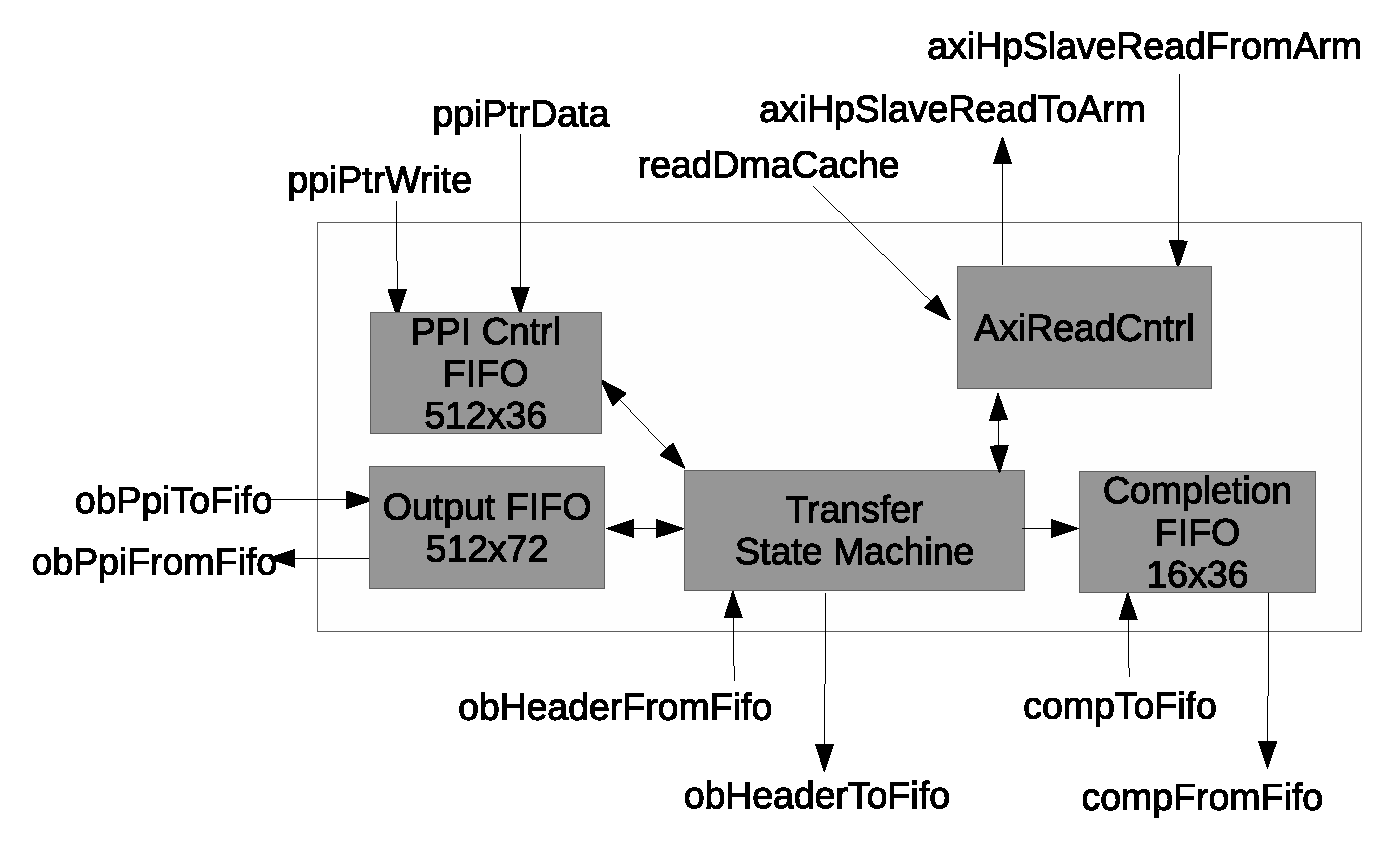
\psfig{file=images/arm_g3_ob_ppi.eps,scale=0.50}
   \caption{Outbound PPI Block Diagram}
   \label{fig:ob_ppi_block}
\end{figure}

\subsubsection{Outbound PPI Transmit Control}

Outbound PPI frame transmission is controlled by the last four 32-bit dual words in the outbound PPI header frame. 
These four words form the outbound PPI transmit descriptor and are not included in the outbound frame. All four
32-bit dual words are ignored for transaction types 0 and 1. The last two dual words are ignored for transaction
types 0, 1 and 2.

The format of the outbound PPI transmit control descriptor is shown in table \ref{tab:ob_ppi_cntrl}.

\begin{table}[H]
\small
\centering
   \begin{tabular}{| l | l | l | l | l | l | } 
      \hline \textbf{DWord} & \textbf{Bits} & \textbf{Name} & \textbf{Description} \\
      \hline 0              & 31:0          & ObAddr        & Outbound frame source address     \\
      \hline 1              & 31:0          & ObLength      & Length of outbound frame in bytes \\
      \hline 2              & 31:4          & CompId        & Id value for completion record.  \\
      \hline 2              & 3:0           & unused        & ignored                           \\
      \hline 3              & 31:4          & unused        & ignored                           \\
      \hline 3              & 3:0           & CompIndex     & Completion FIFO selection index.  \\
                            &               &               & Valid values are 0 - 10.          \\
      \hline
   \end{tabular}
   \caption{Outbound PPI Transmit Descriptor}
   \label{tab:ob_ppi_cntrl}
\end{table}

\subsubsection{Outbound PPI Transmit Completion Record}

When the outbound frame DMA operation is completed, the outbound PPI engine has the ability to add a completion record to one of the 11 
completion FIFOs. The CompEn bit in the outbound transmit control descriptor determines if a completion record is 
generated and the CompIndex field determines which of the 11 FIFOs to route the completion record to. The value written 
to the completion record is defined in the CompId field of the outbound transmit control record. 

The format of the receive completion record is shown in table \ref{tab:ob_ppi_comp}.

\begin{table}[H]
\small
\centering
   \begin{tabular}{| l | l | l | l | l | } 
      \hline \textbf{Bits} & \textbf{Name} & \textbf{Description} \\
      \hline 31:4          & CompId        & Completion ID field from transmit descriptor.                           \\
      \hline 3:1           & Unused        & Read as zero.                          \\
      \hline 0             & Invalid       & Asserted when the completion value is emtpy upon read. \\
      \hline
   \end{tabular}
   \caption{Outbound PPI Transmit Completion Descriptor}
   \label{tab:ob_ppi_comp}
\end{table}

\subsection{AXI Read Controller (ArmRceG3AxiReadCntrl.vhd)}
\label{subsec:ArmRceG3AxiReadCntrl}

Similar to the AXI write control module, the AXI read controller provides arbitration between AXI masters in cases
where more than one read source is attached to a shared AXI bus. It also provides an address FIFO 
between the attached read state machine and the processor's AXI interface. Returned read data is first
passed to a FIFO to decouple flow control which may be originated by the attached read state machine(s) from
the signals on the AXI bus interface.

The AXI read controller supports two modes of operation. The first supports 4 separate write masters when
used in the outbound controller block (see section \ref{subsec:ArmRceG3IbCntrl}). The second supports a single 
master when used in the in the outbound PPI controller (see section \ref{subsec:ArmRceG3ObPpi}).
When only master is attached the arbitration stage is optimized away to reduce latency.

\subsubsection{Axi Read Controller Block Diagram}

The AXI read controller contains an arbitration block which selects between one of 4 possible AXI masters. Address data is 
buffered in a 36-bit x 512 entry FIFO. An address engines converts the address into transactions on the AXI bus. 

\begin{figure}[H]
   \centering
   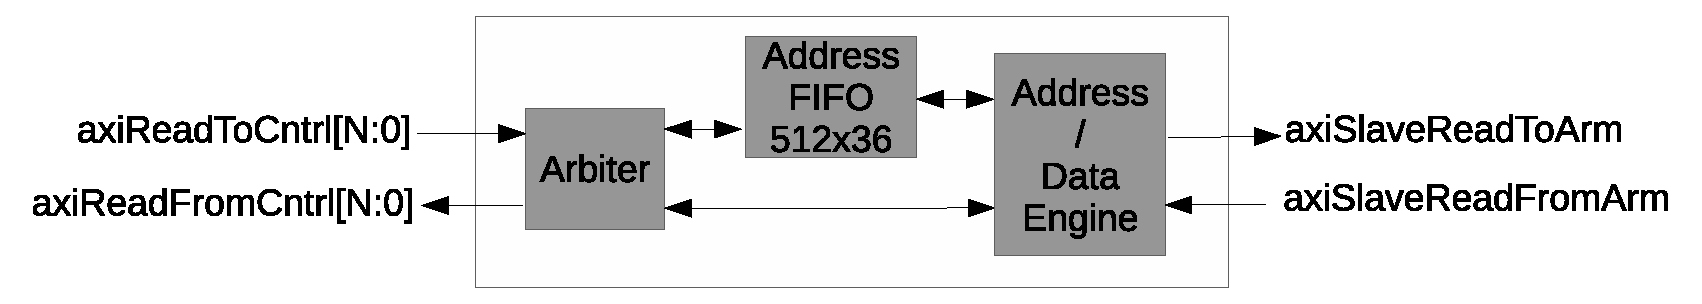
\psfig{file=images/arm_g3_axi_read.eps,scale=0.50}
   \caption{Axi Read Controller Block Diagram}
   \label{fig:axi_read_block}
\end{figure}

\subsection{DMA Completion FIFO Controller (ArmRceG3DmaComp.vhd)}
\label{subsec:ArmRceG3DmaComp}

The purpose of the DMA completion FIFO controller is to accept completion records from the four inbound PPI engines and the four outbound PPI engines. 
Each of the PPI engines has the ability to direct it's completion entries to one of 11 completion FIFOs. Each completion entry is treated independently 
and can be targeted to a different completion FIFO than other completion entries from the same source. 

When a completion FIFOs is non-empty it asserts a ready status bit which can be read over the AXI bus and be configured to trigger an interrupt. 
The mapping of the 11 completion FIFOs to interrupts is described earlier in this document in table \ref{tab:dma_int_mappings}. The contents of
the completion FIFOs are read over the AXI bus. When software reads from the address associated with a completion FIFO the entry at the head of
the queue is returned to software and the contents of the FIFO are advanced. 

The completion engine works by iterating through each of the 8 possible sources, one per clock cycle. When a particular source is selected the
completion record is examined and the destination ID is determined. If the requested destination FIFO is not full the completion entry will 
then be moved to the selected completion FIFO. 


\subsubsection{DMA Completion Block Diagram}

The DMA completion module consists of a completion engine which transfers data from a series of small inbound header and outbound header 
completion FIFOs to one of 9 independent 36-bit x 512 entry completion FIFOs. A read control block allows the 9 completion to be read from
the local bus.

The DMA completion module also contains a single completion free list FIFO. This FIFO can be written to and read from through the local AXI address space. 

\begin{figure}[H]
   \centering
   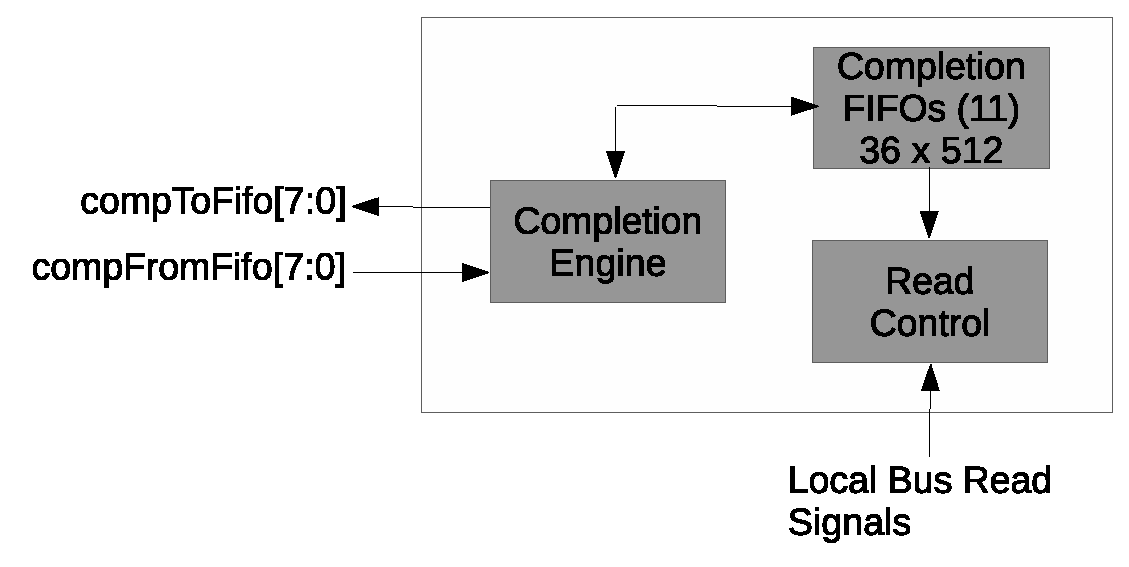
\psfig{file=images/arm_g3_dma_comp.eps,scale=0.50}
   \caption{DMA Completion Block Diagram}
   \label{fig:dma_comp_block}
\end{figure}

\subsection{I2C Controller (ArmRceG3I2c.vhd)}
\label{subsec:ArmRceG3I2c}

The I2C controller block supports the BSI operation by providing a message path between the CPU software and the management I2C bus. Anytime a 
byte is written over the I2C bus the appropriate entry in the I2C BRAM is updated with the data contained in the write. When a complete 32-bit
word is written the FIFO writer block will place the 32-bit value along with the target address in the BSI quad word FIFO. 

A 32-bit value is written over the I2C bus by writing the least significant byte first (offset address 0), followed by the second byte (offset 1)
and third byte (offset 2). When the finally byte (offset 3) is written it's value is combined with the previous three received bytes and added to
the quad word FIFO. Software also has the ability to directly read and write the I2C BRAM. 

The I2C management controller may poll the flow control state of the BSI FIFO by reading from offset address 0x800.

\subsubsection{I2C Controller Block Diagram}

The I2c controller module consists of a I2C slave core which converts I2c bus accesses to local byte transfers. A 2Kbyte dual port block ram 
allows read and write access from either the local bus or the I2C bus. A FIFO write module converts I2C write access to quad word FIFO writes.

\begin{figure}[H]
   \centering
   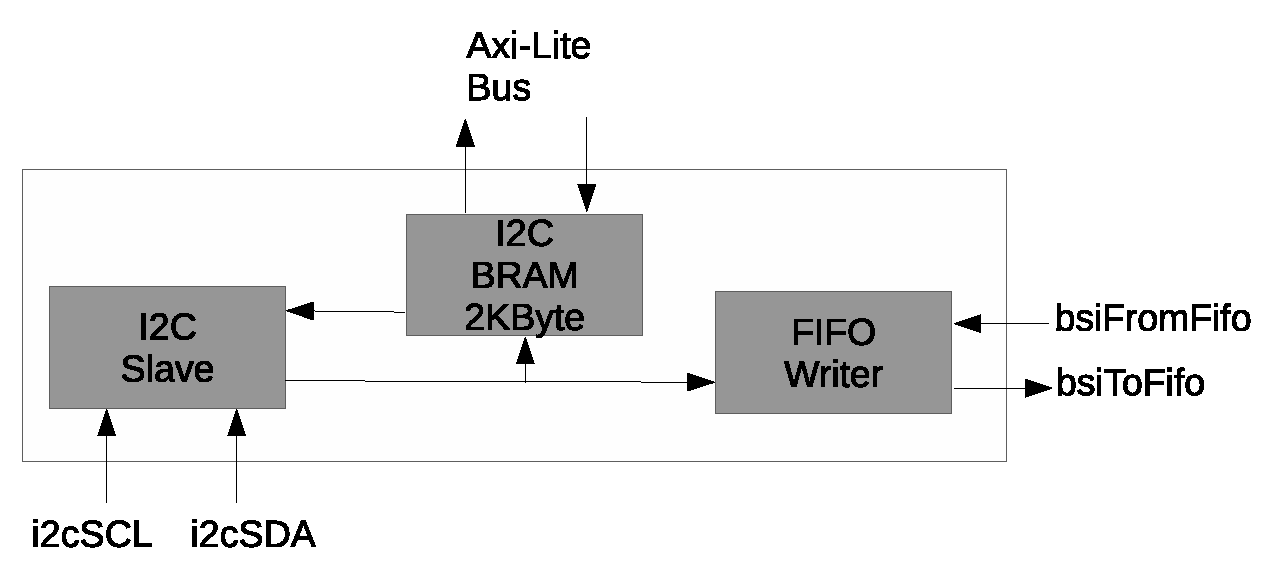
\psfig{file=images/arm_g3_i2c_cntrl.eps,scale=0.50}
   \caption{I2C Controller Block Diagram}
   \label{fig:i2c_cntrl_block}
\end{figure}

\subsubsection{Local Bus Address Space}

RCE software may access the contents of the 2K I2C block ram in the address space 0x8400\_0000 - 0x8400\_07FC.

\subsubsection{I2C Bus Address Space}

The I2C controller may access the contents of the 2K I2C block ram in the address space 0x00 - 0x7FF. 
The BSI Quad Word almost full status appears in bit 0 at address 0x800.
The I2C bus address of the slave device is 0x49.

\subsection{CPU Interface Module (ArmRceG3Cpu.vhd)}
\label{subsec:ArmRceG3Cpu}

The CPU interface module is a wrapper to the processor\_system7\_v4\_02a core provided from Xilinx. 
The interfaces used in the ARM RCE generation 3 core are converted to record types. Unused interfaces are terminated with constants.

Further information and documentation for the processor\_system7 core can be found on the Xilinx website at:
\begin{center}
   \url{http://www.xilinx.com/products/intellectual-property/processing_system7.htm}
\end{center}

\end{document}

